\documentclass[aps,prl,preprint,superscriptaddress,longbibliography,nofootinbib]{revtex4-2}
\usepackage{graphicx}
\usepackage{amsmath,amssymb}
\usepackage{bm}
\usepackage{longtable}
\usepackage{booktabs}
\usepackage[colorlinks=true,linkcolor=blue,citecolor=blue,urlcolor=blue]{hyperref}
\graphicspath{{figures/}}
\newcommand{\um}{\,\mu\mathrm{m}}
\newcommand{\umi}{\,\mu\mathrm{m}^{-2}}
\renewcommand{\thefigure}{S\arabic{figure}}
\renewcommand{\thetable}{S\arabic{table}}
\renewcommand{\thesection}{S\arabic{section}}
\renewcommand{\theequation}{S\arabic{equation}}

\begin{document}

\title{Supplemental Material for ``Localized in-gap eigenstates of a $10^4$-vertex disordered photonic network from direct interior Maxwell eigensolves''}
\author{F. Hern\'andez}
\affiliation{[affiliation to be filled]}
\date{\today}
\maketitle

\tableofcontents

\section{Scope, reproducibility and conventions}
This Supplemental Material is the complete technical record of the two computations behind the main text: the bottom-up $N=1000$ project (delivered 2026-08-14) and the interior $N=10^4$ project (2026-08-17 to 2026-08-31). Every number quoted in either document is listed in \texttt{report/numbers.json} of the repository with the data file it was derived from and the script that derived it; where a number can be recomputed from saved fields or spectra it \emph{was} recomputed for this paper (scripts \texttt{report/scripts/s01}--\texttt{s06}), and the recomputed value is the one printed. Timings, operator-application counts and bake-off metrics are cited from the run records (\texttt{results/*/interior\_report.json}, \texttt{results/exp/*.json}, logs). The pre-registered plans, the four adversarial-verification records and the gate ledger (\texttt{results/gates/gate\_results.json}) are part of the repository. Nothing was re-solved for this paper; all analysis is CPU post-processing of saved data.

\emph{Units.} $\lambda=(\omega/c)^2$ in $\umi$; $\nu=\omega a/2\pi c=\sqrt{\lambda}\,a/2\pi$ with $a=L/5=2.288\um$ for $N=1000$ and $a=L/1250^{1/3}=2.288\um$ for $N=10^4$ (the same density-equivalent 8-vertex cell). Relative gap widths are $\Delta\nu/\nu=2(\omega_2-\omega_1)/(\omega_2+\omega_1)$. Band numbering is MPB's: bands 1--2 are the $\omega=0$ modes at $\Gamma$, so the $n$-th eigenvalue returned by the transverse solver is band $n+2$. A $\pm2$ ambiguity of this convention against the original cluster montage's labelling is undecidable from local artefacts and is carried as an open item. All residuals are relative, $\|\Theta x-\lambda x\|/\|\Theta x\|$.

\section{Structure generation and rasterization}
\subsection{Networks}
The $N=1000$ network is the reference LSU structure of Ref.~\cite{Sellers2017} (its gap between bands $N/2$ and $N/2+1$ follows the band arithmetic of the parent srs/gyroid crystal~\cite{Lu2013}) as distributed with the parent project (file \texttt{N1000\_lsu\_example\_ends.txt}: 1653 rod rows, i.e.\ the 1500 edges of a trivalent 1000-vertex network plus periodic duplicates of face-crossing segments; mean rod length $0.800\um$, median $0.801\um$; $L=11.44\um$). The $N=10^4$ network (\texttt{Structures/20260701\_N10000\_lsu\_generated.txt}: 15\,704 rows, mean rod length $0.801\um$) was generated with the same protocol at the same vertex density, $L=(N/1000)^{1/3}\times11.44\um=24.6467\um$ ($L_{10^4}/L_{10^3}=2.15443=10^{1/3}$). The LSU family constant $d_0=0.8\um$ is the target rod length.

\subsection{Rasterizer (montage convention)}
\texttt{eigenfns/structure.py::rasterize\_penlike} reproduces the parent notebook's \texttt{create\_permittivity\_grid\_penlike} algorithmically: right circular cylinders of radius $r$ are built in an unwarped space $(x,y,z'=z/s)$ and the global warp $z=s\,z'$ stretches them along $z$, so the cross-section perpendicular to a rod at angle $\theta$ from $\hat z$ is an ellipse with semi-axes $r$ and $r\sqrt{\cos^2\theta+s^2\sin^2\theta}$ (the direct-laser-writing ``pen'' sweep; near-vertical rods stay circular). Membership is tested at voxel centres with flat caps ($0\le t\le \ell$ along the axis); a voxel is $\varepsilon_{\rm rod}$ if its centre lies inside any rod, else 1---binary voxels, no subpixel averaging (MPB-style smoothing~\cite{Farjadpour2006,Kottke2008} is deliberately not applied, for fidelity to the reference montage). The implementation is bit-identical to the notebook's at $64^3$ (0 differing voxels) and differs in 5 of $16.7\times10^6$ voxels at $256^3$ (float32 vs float64 boundary arithmetic).

Decorations: \emph{elliptical} (montage convention) $r=0.2252\um$, $s=2.5$, $n=2.9275$, $\varepsilon=8.5703$: ff $=0.2173$ ($64^3$), $0.2172$ ($128^3$), $0.2172$ ($256^3$). \emph{Circular} $r=0.331836\um$, $s=1$, $n=2.9$, $\varepsilon=8.41$: the radius was bisected on the $N=10^4$ structure to ff $=0.2200$ at $256^3$ (terminating at $|{\rm ff}-0.22|=4\times10^{-6}$); it gives $0.22011$ at $192^3$, $0.22006$ at $160^3$, and $0.2191$ on the $N=1000$ structure at $128^3$ (gate I7: $22.0\pm0.5\%$, PASS). Voxel sizes: $0.0894\um$ ($N=1000$, $128^3$; 11.2 vox/$\mu$m; circular rod diameter 7.4 voxels, elliptical minor diameter 5.0) and $0.1284\um$ ($N=10^4$, $192^3$; 7.79 vox/$\mu$m, 70\% of the $N=1000$ resolution; rod diameter 5.2 voxels).

\subsection{The boundary seam and its fix}
The rod files list periodic duplicates only for segments that \emph{cross} a face; a rod whose \emph{radius} pokes through a face is not wrapped, so its wrap-image voxels are missing. Measured on the $N=10^4$ $192^3$ grid: filling fraction by depth from a face $d=0,1,2$: $0.1975$, $0.2144$, $0.2201$; interior ($d\ge10$): $0.2211$---an $10.7\%$ material deficit in the outermost shell (11.8\% at $256^3$). The $N=1000$ grids carry the same seam ($12.8\%$ elliptical, $11.3\%$ circular at $128^3$). In a gapped medium this thin low-index sheet is a planar defect and hosts defect states: four of the ten $N=10^4$ in-gap states carry 18.2, 23.6, 43.7 and 42.1\% of their $\varepsilon|E|^2$ in the outer 2-voxel shell (6.12\% of the volume; enhancements 3.0--7.1$\times$), and three of them peak at a voxel with two coordinates on box faces. Twenty of the 133 window modes have shell enhancement $>2$; the bulk-localized in-gap candidates have 2.5--10.5\% ($0.4$--$1.7\times$). The $N=1000$ windows also contain modes with shell enhancement up to $3.95\times$ (elliptical) and $3.43\times$ (circular), although both $N=1000$ gaps are empty (Fig.~\ref{figS_seam}).

The fix, \texttt{periodic=True}, assigns voxels by minimum image so each rod contributes its full volume wherever it sits. It changes 5528 voxels of the $192^3$ grid (0.078\%), every one within 3 voxels of a face; the outer-shell ff becomes 0.2177 and the global ff $0.22089$ ($0.22058$ for $N=1000$ circular at $128^3$, 0.15\% of voxels). It is a convention change relative to the reference montage and lives behind a flag; the production window was solved with the montage convention, and the gap window was \emph{re}-solved with the fix (Sec.~\ref{sec:seam}).

\begin{figure}
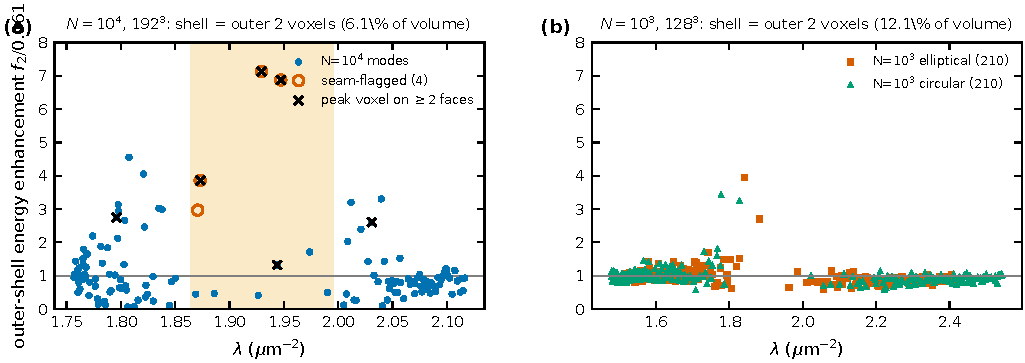
\includegraphics[width=\textwidth]{figS_seam}
\caption{Outer-2-voxel-shell energy fraction divided by the shell volume fraction for every window mode. (a) $N=10^4$, $192^3$: the four seam-flagged in-gap states (open red) and the modes whose peak voxel has two coordinates on a face (crosses). (b) The two $N=1000$ windows at $128^3$ (shell volume 12.1\%).}
\label{figS_seam}
\end{figure}

\section{Operator}
$\Theta\bm H=\nabla\times\varepsilon^{-1}\nabla\times\bm H$ in MPB's transverse plane-wave representation~\cite{Johnson2001}: every field is a pair of complex amplitudes on the two transverse unit vectors $(\hat t_1,\hat t_2)\perp(\bm k+\bm G)$ for every reciprocal vector on the grid, so $\nabla\cdot\bm H=0$ is exact by construction and the curl is the $2\times2$ block $|\bm k+\bm G|\,\sigma_y$ on each plane wave. One application: spectral curl $\to$ Cartesian $\to$ inverse FFT $\to$ multiply by $\varepsilon^{-1}(\bm r)$ $\to$ FFT $\to$ project the curl back: six 3-D FFTs. At $k=\Gamma$ the $\bm G=0$ plane wave has no transverse pair; both its amplitudes are zeroed, which removes the two $\omega=0$ modes exactly and makes $\Theta$ positive definite on the remaining space (dimension $2G^3-2$). With real scalar $\varepsilon$ the operator is real symmetric on real fields. Validation of the operator itself: against the analytic homogeneous spectrum at $G=8$ the maximum relative error is $2.6\times10^{-7}$ (complex64) with null dimension exactly 2; against an independent dense fp64 three-component construction the nonzero spectra agree to $1.2\times10^{-7}$ and the Hermiticity residual is $5.6\times10^{-8}$.

Measured cost (complex64, RTX 4080 Laptop 12~GB, chunked application): $2.7$~ms/vector at $128^3$ ($N=1000$); $23.2$ ($192^3$), $38.2$ ($224^3$), $53.9$ ($256^3$), $79.2$~ms ($288^3$) for $N=10^4$ (Table~\ref{tab:timing}). $\lambda_{\max}$ (two-seed Lanczos upper estimate $\times1.05$): $4633.6$ ($128^3$, $N=1000$), $2208.9$ ($192^3$), $3030.7$ ($224^3$), $3974.6$ ($256^3$), $5055.9$ ($288^3$). One vector is $2G^3$ complex64 $=0.113$~GB at $192^3$, $0.268$~GB at $256^3$.

\begin{table}
\caption{Operator application time and spectral extent per grid ($N=10^4$, circular decoration; \texttt{results/exp/n10k\_G*\_timing.json}).}
\label{tab:timing}
\begin{tabular}{@{}lrrrr@{}}
\hline\hline
 grid & vox/$\mu$m & $\Theta$ apply (ms/vector) & $\lambda_{\max}$ ($\mu$m$^{-2}$) & vector (GB) \\
\hline
 $192^3$ & 7.79 & 23.2 & 2209 & 0.113 \\
 $224^3$ & 9.09 & 38.2 & 3031 & 0.180 \\
 $256^3$ & 10.39 & 53.9 & 3975 & 0.268 \\
 $288^3$ & 11.69 & 79.2 & 5056 & 0.382 \\
\hline\hline
\end{tabular}

\end{table}

\section{Bottom-up solver ($N=1000$)}
\subsection{Algorithm}
Deflated block LOBPCG~\cite{Knyazev2001,Duersch2018} (\texttt{eigenfns/solver.py}): blocks of $m=32$ with 12 guard vectors, warm-started from the previous block's guard Ritz vectors; MPB's transverse-projection preconditioner~\cite{Johnson2001} (Eq.~14 there; the same six-FFT cost as $\Theta$; it reduced per-block iteration counts to 18--72 and made them resolution-stable); SVQB orthonormalization with drop threshold $10^{-5}$ (the fp32 Gram noise floor); all small dense algebra (Gram eigendecompositions, Rayleigh--Ritz) in fp64 on the host; $\Theta X$ recomputed every iteration (tracked products drift by $\sim10^{-3}\|\Theta W\|$ in complex64); re-deflation against the locked set every iteration; rank-dropped rows penalized on the Rayleigh--Ritz diagonal; fixed array shapes throughout (XLA recompiles otherwise); chunk-assembled Rayleigh--Ritz; host-resident locked set streamed in $\approx0.75$~GB chunks with a barrier per chunk; per-block checkpointing with automatic resume. Locking tolerance: relative residual $\le10^{-4}$ (Weyl: $\Delta\omega/\omega\le5\times10^{-5}$ unconditionally; the measured interior error is $\sim4\times10^{-6}$).

\emph{TF32.} On Ada GPUs XLA's default runs fp32 matmuls in TF32 (10-bit mantissa); measured at $64^3$ the Gram/rotation accuracy floors at $\sim10^{-3}$ and block residuals plateau at $\sim7\times10^{-3}$. Every matmul/tensordot carries \texttt{precision=HIGHEST}. FFTs are unaffected. A second precision trap, found in adversarial round 3 of the interior project, is described in Sec.~\ref{sec:rayleigh}.

\subsection{Gates G1--G9}
Pre-registered on 2026-08-13 (thresholds verbatim in \texttt{plans/2026-08-13\_preregistered\_plan.md}); outcomes in Table~\ref{tab:gatesG}. The judge protocol for parity is: MPB 1.11.1 reads our $\varepsilon$ grid from file (\texttt{epsilon-input-file}), we read back MPB's \texttt{-epsilon.h5} and solve on \emph{that} grid, so the two codes see the identical discrete problem.

\begin{table}
\caption{$N=1000$ gates (pre-registered criteria; recomputed values where the data allow).}
\label{tab:gatesG}
\begin{tabular}{@{}p{2.2cm}p{5.3cm}p{2.0cm}p{7.2cm}@{}}
\hline\hline
gate & registered test / threshold & outcome & measured \\ \hline
G1 crystal parity & srs cell $+$ $2\times2\times2$ supercell, $\Gamma$ $+$ 3 $k$-points vs MPB, $\Delta\omega/\omega\le10^{-4}$ & \textbf{not run} & never executed as registered; production claims are $\Gamma$-only; no $k\ne\Gamma$ validation exists. The identical-grid protocol was validated on the disordered structure instead (G3) \\
G2 literature & srs at Sellers's parameters, gap $28.06\pm1.5$~pp & PASS & 27.97\% \\
G3 parity & 300 bands, $64^3$, $\Delta\omega/\omega\le10^{-4}$ per band & PASS & 298 bands: max $8.95\times10^{-6}$, median $1.42\times10^{-6}$ (MPB tol $10^{-7}$, fp64; 2\,h\,22\,m CPU vs 33\,min for our solver on CPU) \\
G3w parity & 660 bands, $64^3$ & PASS & 658 bands: max $3.55\times10^{-5}$, median $1.39\times10^{-6}$; $+2$ band alignment unique \\
G4 degeneracies & clusters ($\Delta\lambda<10^{-3}\lambda$) compared as subspaces, principal-angle cosine $\ge0.99$ & PASS (scope-limited) & 6 low-lying clusters (bands $\le30$), min cosine 0.999986; window clusters (64\% of adjacent pairs qualify) were not field-compared \\
G5 convergence & $\omega(G)$ for bands \{398,450,500,501,550,607\} at 96/128/160$^3$ (160$^3$ not run; 64$^3$ substituted) and $\omega$(tol) sweep (not run); monotone & \textbf{FAIL} as registered & 5/6 bands monotone, worst Richardson residual 0.23\% at $128^3$; band 500 non-monotone, spread 0.274\% ($55\times$ the tol-$10^{-4}$ Weyl bound, $1800\times$ the measured solver--MPB error): rasterization-limited (Fig.~\ref{figS_g5}) \\
G6 completeness & (a) monotone locking; (b) deflated-probe KPM count of missed eigenvalues, $=0$ with s.e.\ $\le0.5$ & PASS below the gap (amended) & (a) zero violations; (b) at mid-gap, degree 8000: $0.21\pm0.02$ (Jackson-tail bias, inconsistent with a missed band). First version (threshold at band 619, degree 800) read 86.6 phantom missing bands---a smearing artefact, recorded. Above-gap completeness rests on monotone locking $+$ $64^3$ parity \\
G7 residuals & rel-res $\le10^{-4}$; orthonormality $\le10^{-3}$ & PASS & worst $9.78\times10^{-5}$; full $210\times210$ window Gram $|G-I|_{\max}=1.2\times10^{-5}$; window-vs-locked cross overlap $\le9\times10^{-8}$ \\
G8 montage & gap must straddle 500|501; regenerate the 210-tile montage & PASS & gap at 500|501, $\Delta\nu/\nu=2.08\%$ at $128^3$; montage regenerated (Fig.~\ref{figS_montage_ell}); disclosures: the 114|115 shell jump (2.37\%) is larger than the gap; width non-monotone 2.35/1.93/2.08\% \\
G9 precision & c64 vs c128 at $48^3$, 96 bands, $\le10^{-4}$ & PASS & $2.44\times10^{-7}$ \\
\hline\hline
\end{tabular}
\end{table}

\begin{table}
\caption{Parity and precision tests (recomputed from the saved spectra; $\Delta\omega/\omega$ unless stated).}
\label{tab:parity}
\begin{tabular}{@{}llrrr@{}}
\hline\hline
 test & grid / bands & $n$ & max $\Delta\omega/\omega$ & median \\
\hline
 MPB parity (32$^3$, 150 bands, tol $10^{-9}$) & & 148 & $4.3\times10^{-6}$ & $8.6\times10^{-7}$ \\
 G3: MPB parity (64$^3$, 300 bands, tol $10^{-7}$) & & 298 & $9.0\times10^{-6}$ & $1.4\times10^{-6}$ \\
 G3w: MPB parity (64$^3$, 660 bands) & & 658 & $3.5\times10^{-5}$ & $1.4\times10^{-6}$ \\
 G9: c64 vs c128 (48$^3$, 96 bands) & & 96 & $2.4\times10^{-7}$ & -- \\
 I1: interior vs bottom-up ($N=1000$, 128$^3$; $\Delta\lambda/\lambda$) & & 55 & $2.4\times10^{-7}$ & $6.3\times10^{-8}$ \\
 I4: interior vs bottom-up ($N=1000$ circ.; $\Delta\lambda/\lambda$) & & 216 & $4.1\times10^{-7}$ & $9.8\times10^{-8}$ \\
\hline\hline
\end{tabular}

\end{table}

\subsection{The gap at $64^3$ depends on the $\varepsilon$ representation}
A new observation made while recomputing the parity numbers: on the MPB judge grid (MPB's trilinear read-back of our binary $64^3$ grid), both codes agree to $3.5\times10^{-5}$ but the elliptical 500|501 spacing is only $0.60\%$ and the largest spacing in the window sits at 501|502 ($0.83\%$), whereas on our binary $64^3$ raster the gap is at 500|501 with $2.35\%$ (501|502: 0.61\%). Bands 498--503 differ between the two $\varepsilon$ representations by $-1.4\%$ to $-3.3\%$. The binary raster is the montage convention and is what all production results use; at $128^3$ the 500|501 spacing is $9.6\times$ the median of its twenty neighbours (elliptical) and $26\times$ (circular), so the statement is robust there, but at $64^3$ ``the gap is at 500|501'' is a statement about the binary-voxel convention. This is the same rasterization sensitivity that failed G5.

\begin{figure}
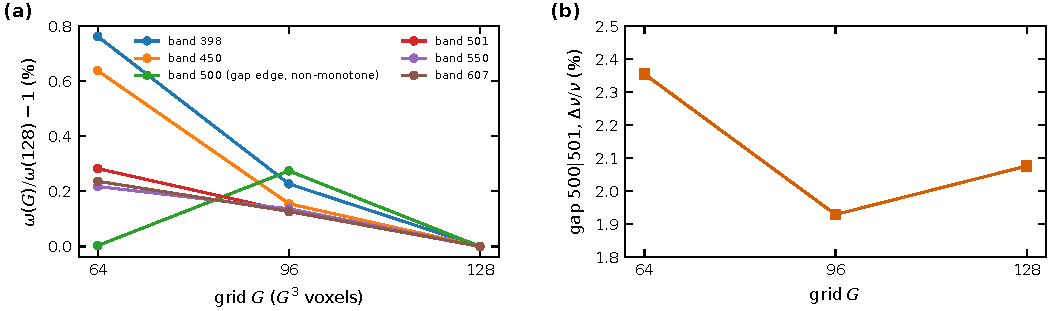
\includegraphics[width=\textwidth]{figS_g5}
\caption{G5: (a) $\omega(G)/\omega(128^3)-1$ for the six registered bands at $64^3/96^3/128^3$; band 500 (gap edge) is non-monotone. (b) The elliptical gap width vs grid.}
\label{figS_g5}
\end{figure}

\subsection{Performance}
611 bands at $128^3$ (elliptical): 19\,908~s $=5$\,h\,32\,m, 31 blocks with 23--72 iterations each, $\approx1.3\times10^{5}$ operator applications; the registered target was 4~h (missed; inside the 12~h cap). Circular decoration, same window: 8876~s, $6.97\times10^{4}$ applications. $96^3$: 6426~s. 680 bands at $64^3$: 942~s. Against MPB at matched work (300 bands, $64^3$): $\sim18\times$ in wall clock, with stated confounds (MPB's tolerance $10^{-7}$ vs our $10^{-4}$, fp64 vs complex64, single process vs a 32-thread host); the tolerance-matched, core-for-core advantage is likely single-digit.

\section{Interior solver ($N=10^4$)}
\subsection{Why new machinery}
Extrapolating the production profile to the $\approx5150$ bands below the $N=10^4$ gap at $256^3$: locked-set storage $5150\times0.268$~GB $=1.38$~TB ($12\times$ RAM $+$ disk), deflation time $O(100)$~days (order-of-magnitude; the $n^2$ regime is not yet visible at $N=1000$ scale), pure matvec time 16.4~h. A bottom-up Chebyshev filter hits the same storage wall.

\subsection{Kernel polynomial method}
Stochastic Chebyshev moments $\mu_k=\langle z|T_k(B)|z\rangle$ with $B=(2\Theta-\lambda_{\max})/\lambda_{\max}$, Rademacher probes $z$ restricted to the transverse space, even/odd doubling (degree-$p$ moments from $p/2$ applications), Jackson kernel~\cite{Weisse2006}. Counting function $N(\lambda_b)=\sum_k g_k\mu_k c_k(x_b)$ with $c_k$ the Chebyshev coefficients of the step; per-probe values give the standard error. Jackson width at position $\lambda$: $\sigma(\lambda)=\pi\sqrt{1-x^2}\,\lambda_{\max}/2p$.

\emph{Validation on $N=1000$} (same $128^3$ grid as the exact 611-band spectrum; degree 8000, 16 probes, 731~s): window count $213.3\pm2.6$ vs exact 210; count below mid-gap $501.5\pm2.7$ vs exact 498; total-trace normalization exact. The gap edges from the 10\%/20\% criteria, $[1.861,1.974]$/$[1.830,2.013]$ on a uniform $5\times10^{-4}$ grid, bracket the exact $[1.883,1.963]$ within the smearing width $0.037$, i.e.\ KPM edges carry a criterion-dominated systematic of $\pm0.02$--$0.03$ (Fig.~\ref{figS_kpm}).

\emph{$N=10^4$} ($256^3$, degree 12\,000, 12 probes, $\lambda_{\max}=3974.6$, 8477~s; Jackson width at the gap $0.023$): the count below $\lambda=1.957$ is $5010.3\pm12.5$ ($0.501$ bands/vertex; $5008.3\pm12.6$ below the bracket centre 1.930), placing the gap between MPB bands $\approx5012|5013\pm13$. The registered nominal gap is the interval where the smoothed DOS is below 160 states per unit $\lambda$, $[1.864,1.996]$ ($\Delta\nu/\nu=3.41\%$); the 5\% and 20\% criteria of the project (thresholds 80 and 320) give $[1.885,1.968]$ (2.14\%) and $[1.837,2.022]$ (4.78\%). [The project's script normalizes by a ``local median'' DOS whose grid dependence we could not reproduce exactly; the registered brackets are reproduced to the grid step by the absolute thresholds, which is how we state them.] Window populations: $139.3\pm2.8$ in the production window $[1.757,2.117]$, $317.1\pm5.1$ in $[1.71,2.19]$, $69.2\pm1.5$ / $66.1\pm2.4$ in $S_{\rm below}$/$S_{\rm above}$, $4.87\pm0.41$ in $S_{\rm gap}=[1.925,1.985]$, $11.18\pm0.58$ in the bracket, $3.80\pm0.38$ in the certifying sub-interval $[1.9063,1.9606]$. These are stochastic errors only: the Jackson-smoothed count of an interval is biased by $\approx(\sigma^2/2)\rho'$ at each edge, and both production-window edges sit on steep shoulders ($\rho=1281$ and $996$ states per unit $\lambda$, $\rho'=-1.9\times10^4$ and $+1.1\times10^4$), giving a predicted bias of $+7.7$ states (project record: $+7.5\pm0.3$), so the $139$ vs $133$ comparison is \emph{not} a completeness statement (Sec.~\ref{sec:complete}); on the $N=1000$ calibration six nested gap-straddling windows all have positive error. The same bias makes the absolute tile labels 4942--5074 read $\approx4.5$ low; the count of 133 is exact, the absolute index is not certified beyond $\pm13$.

\begin{figure}
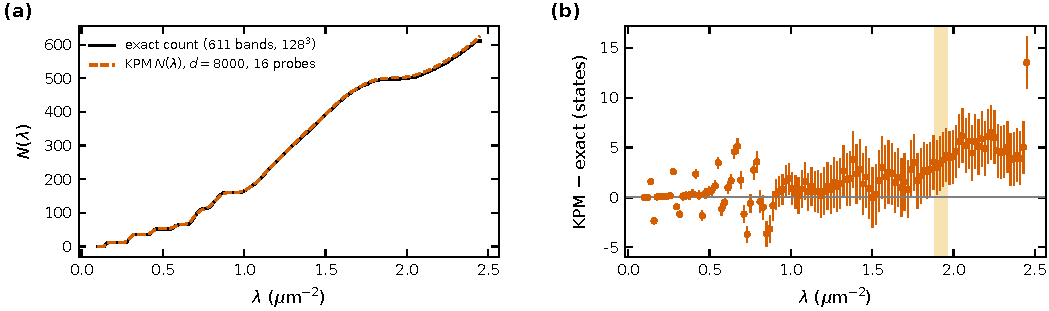
\includegraphics[width=\textwidth]{figS_kpm_validation}
\caption{KPM validation on $N=1000$: (a) counting function vs the exact 611-band spectrum; (b) difference (states), with the exact gap shaded.}
\label{figS_kpm}
\end{figure}
\begin{figure}
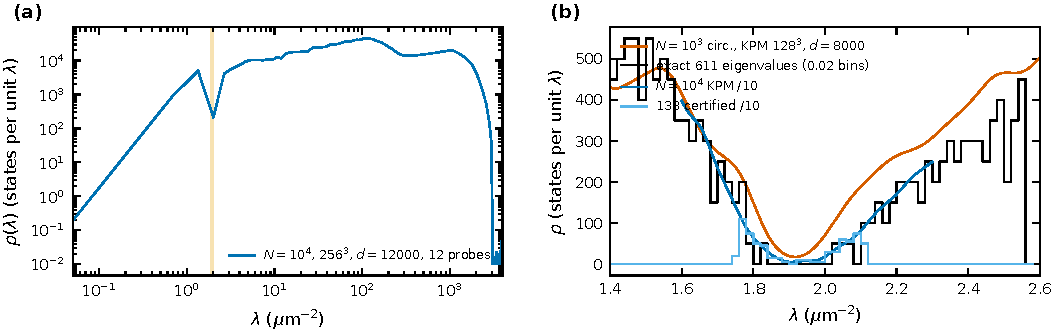
\includegraphics[width=\textwidth]{figS_dos_full}
\caption{(a) Full-bandwidth KPM DOS of the $N=10^4$ structure. (b) The gap region: $N=1000$ circular KPM and exact histogram; $N=10^4$ KPM and the histogram of the 133 certified eigenvalues (both scaled by 1/10).}
\label{figS_dosfull}
\end{figure}

\subsection{Bandpass filter and two-stage subspace iteration}
The bandpass filter is the Jackson-damped Chebyshev expansion of the indicator $1_{[\lambda_{\rm lo},\lambda_{\rm hi}]}$, built as the difference of two step expansions and accumulated during the three-term recurrence (\texttt{eigenfns/interior.py::bandpass\_coeffs}, \texttt{\_apply\_cheb\_poly}): $Y=\sum_k c_k T_k(B)X$, one $\Theta$ application per degree, chunk re-normalized. The transition width scales as $\delta\lambda_t\approx\pi\sqrt{\lambda\lambda_{\max}}/p$; at $192^3$ this is $\approx0.017$ at degree 12\,000 ($\approx27$ states per edge in the bulk) and $\approx0.0086$ at 24\,000. Two stages: \emph{build} at degree 3000--4000, two outer iterations from random starts with $m=1.5\times$ the KPM-predicted population, then \emph{polish} with the same filter at degree 12\,000 on the (trimmed) basis, up to 4--6 outer iterations; the measured residual damping per polish outer was $\times12$ at production against $\times0.62$ for an undersized basis at low degree, which is why two stages beat one. The basis is host-resident and streamed in $\le8$-vector chunks through every stage (filter, SVQB, Rayleigh--Ritz assembly, rotation, residuals); the hosted path matches the device path to $\Delta\lambda\le4.5\times10^{-8}$ and costs $\approx1.5\times$ the raw matvec time. Extraction is exclusively \texttt{rr\_extract}: SVQB orthonormalization, fp64 Rayleigh--Ritz on the \emph{original} $\Theta$, per-pair residuals on $\Theta$; pairs failing $10^{-4}$ are never reported. Ghosts are therefore excluded by construction; zero ghosts were observed in every run of every method. Cross-slice duplicates are identified by eigenvector overlap ($>0.5$), never by eigenvalue proximity.

\subsection{Bake-off}
On a 50-band interior slice of the exact $N=1000$ spectrum (0-based indices 473--522 $=$ MPB bands 476--525, $\lambda\in[1.711,2.146]$, $\sigma=1.9229$; relative slice width $9.4\times10^{-5}$ of $\lambda_{\max}$, close to the $N=10^4$ ratio $1.2\times10^{-4}$) four arms were run at $128^3$ (Table~\ref{tab:bakeoff}, Fig.~\ref{figS_bakeoff}). Folded-spectrum LOBPCG on $(\Theta-\sigma)^2$ with the Wang--Zunger squared-kinetic preconditioner~\cite{Wang1994,Vomel2008} locked 20 vectors at maxit 200 with folded Rayleigh quotients $\mu\in[0.096,0.279]$ while all 50 targets have $\mu\le0.0497$: no preconditioner grips the $\varepsilon$-structure-dominated low spectrum (the ESCAN kinetic-diagonal analogy does not transfer); an earlier residual-based diagnosis of this failure was itself refuted in adversarial round 1 and replaced by the $\mu$-trajectory argument. Shift-invert subspace iteration with preconditioned MINRES inner solves was tolerance-starved (inner iterations at maxit 150/150; median residual 0.18), reproducing the published verdict of Ref.~\cite{Vomel2008}. One-stage bandpass at degree 3300 captured the subspace (50/50 within $2\times10^{-3}$) but damped residuals only $\times0.62$ per outer. (A filtered-Lanczos alternative~\cite{FangSaad2012} was not run: its stored basis of 2.5--5$\times$ the target count exceeds host memory at $192^3$.) Two-stage bandpass verified 24 pairs at $10^{-3}$ within the budget, the remaining 26 (slice-edge and gap-edge pairs) still descending; the lesson (basis must be $\ge1.5\times$ the population) set the production oversampling. Five variants of an expansion-Rayleigh--Ritz polish (LOBPCG-style, filtered residual expansion) were unstable at scale (interior-Ritz ghost instability) and abandoned.

\begin{table}
\caption{Bake-off on the 50-band $N=1000$ slice (\texttt{results/exp/bakeoff\_*.json}, \texttt{.log}). ``Verified'' = residual $\le10^{-3}$ on $\Theta$ and matched to a reference eigenpair. The two-stage wall time is the polish legs; its build is the one-stage row.}
\label{tab:bakeoff}
\begin{tabular}{@{}p{3.1cm}p{4.2cm}rrrrp{4.6cm}@{}}
\hline\hline
Method & Configuration & verified & ghosts & $\Theta$-applies & wall (s) & Failure mode / note \\
\hline
Bandpass ChebSI, one stage & $m=80$, $d=3300$, 3 outers & 0/50 & 0 & 792,528 & 7,109 & subspace captured 50/50 to $2\times10^{-3}$; med. res.\ $6.6\to4.2\to2.5\times10^{-2}$ \\
Two-stage bandpass (build\,+\,polish) & build $d=3300$ $m=80$ $\times2$, trim 56, polish $d=8000$ $\times6$ & 24/50 & 0 & 3,217,088 & 18,464 & 26 unconverged = slice-edge/gap-edge pairs still descending; trim-limited ($1.12\times$ oversampling) \\
Shift-invert PMINRES SI & $m=64$, inner tol $10^{-2}$, maxit 150, 2 outers & 0/50 & 0 & 32,336 & 441 & inner solves hit maxit (150/150); med. res.\ $1.8\times10^{-1}$ \\
Folded-spectrum LOBPCG & $m=32$, WZ preconditioner $\alpha^2\in\{0.05,1,20\}\sigma^2$ & 0/50 & 0 & -- & 629 & first block locked 20 at maxit 200 with folded $\mu\in[0.096,0.279]$ vs targets $\mu\le0.0497$ \\
Expansion-RR polish (5 variants) & on the two-stage build subspace & 0/50 & 0 & -- & -- & med. res.\ $4.2\times10^{-2}\to0.9$ in one sweep; continuity/strip variants oscillate $7$--$23\times10^{-3}$ \\
\hline\hline
\end{tabular}

\end{table}
\begin{figure}
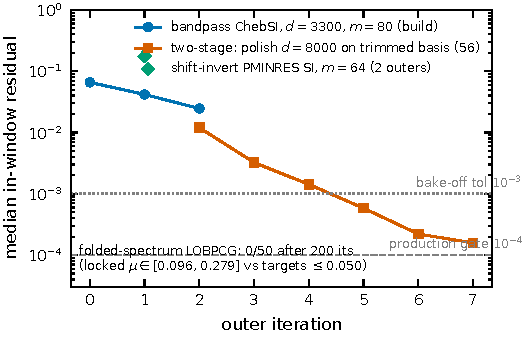
\includegraphics[width=0.6\textwidth]{figS_bakeoff}
\caption{Bake-off: median in-window residual vs outer iteration.}
\label{figS_bakeoff}
\end{figure}

\subsection{The Rayleigh-normalization correction}\label{sec:rayleigh}
Adversarial round 3 (2026-08-25) found that \texttt{rr\_extract} reported the Ritz value as $\langle x,\Theta x\rangle$ without dividing by $\|x\|^2$, while SVQB in blocked fp32 leaves $\|x\|^2-1=+2.8\times10^{-5}$ ($128^3$) and $+4.7\times10^{-5}$ ($192^3$; range $4.4$--$6.5\times10^{-5}$ over the 133 modes)---blocked fp32 accumulation over millions of positive terms under-estimates the Gram diagonal, so the vectors come back slightly over-normalized. Every eigenvalue was biased high by that relative amount. The fp64 check shows the eigenvalue error correlated with $\|x\|^2-1$ at $r=0.969$ (Fig.~\ref{figS_res}b), and dividing it out improves the I1 ground-truth parity from $2.85\times10^{-5}$ to $2.35\times10^{-7}$ ($121\times$). The trap: the same check in fp32 gives the wrong sign and magnitude ($-3.4\times10^{-4}$), because an fp32 sum over $4.2\times10^6$ terms carries its own $\sim10^{-4}$ error. The code was fixed, and all saved eigenvalues were corrected retroactively as $\lambda_{\rm corr}=\lambda_{\rm raw}/\|x\|^2$ with fp64 norms of the saved vectors (\texttt{scripts/exp/fix\_rayleigh\_norm.py}; originals kept as \texttt{window\_eigenvalues\_raw.npy}, norms as \texttt{window\_norms.npy}); this is exactly the Rayleigh quotient of the same vector, so no re-solve was needed. Effects: a uniform shift of $-4.7\times10^{-5}$ relative ($9\times10^{-5}$ absolute at $\lambda\approx1.94$) against a median level spacing of $1.4\times10^{-3}$; no gap, spacing, localization or DOS comparison moves. The reported residuals were computed with the raw $\lambda$ and carry a floor of the same size ($r_{\rm rep}^2=r_{\rm true}^2+\delta^2$): the worst reported residual $8.7\times10^{-5}$ is $\approx5.9\times10^{-5}$ after the correction (direct fp64 recomputation in the ledger: $5.88\times10^{-5}$), so about half the residual budget was being spent on the bug; no state was lost to it (zero in-window unconverged pairs in all three slices). The correction was independently confirmed twice: a fresh interior solve of the circular $N=1000$ decoration with the fixed code lands at $4.1\times10^{-7}$ against a different bottom-up reference; and the two states found by two different slices, whose raw eigenvalues differed by $1.42\times10^{-6}$ and $1.73\times10^{-6}$, agree to $7.7\times10^{-9}$ and $1.2\times10^{-8}$ after dividing each by its own $\|x\|^2$.

\begin{figure}
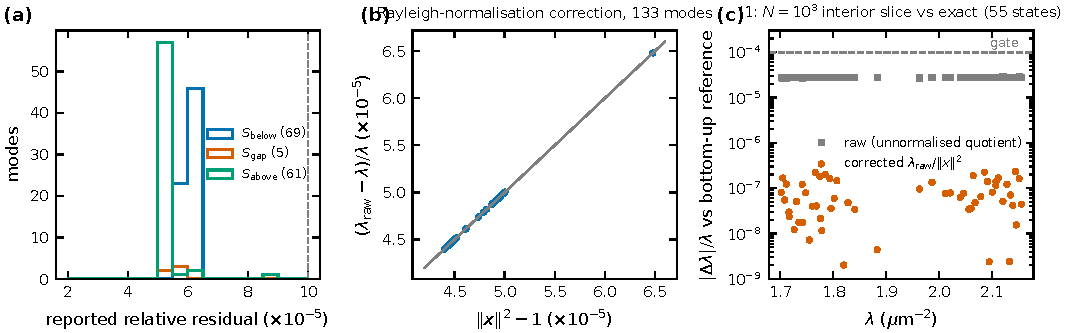
\includegraphics[width=\textwidth]{figS_residuals_rayleigh}
\caption{(a) Reported residuals of the three production slices. (b) Relative eigenvalue shift of the correction vs $\|x\|^2-1$ (line: identity). (c) I1: per-state $|\Delta\lambda|/\lambda$ of the interior slice against the exact bottom-up eigenvalues, raw and corrected.}
\label{figS_res}
\end{figure}

\subsection{Production runs}
Table~\ref{tab:runs} lists every interior run. The production window $[1.757,2.117]$ was descoped at registration from the $\sim300$-band window $[1.71,2.19]$ (10--15 GPU-days at $256^3$) to $\approx139$ bands at $192^3$; it was solved as $S_{\rm below}=[1.757,1.930]$ ($m=104$) and $S_{\rm above}=[1.980,2.117]$ ($m=100$), plus the Amendment-A2 slice $S_{\rm gap}=[1.925,1.985]$ ($m=16$) added after the first in-gap states appeared. $69+5+61=135$ pairs, 133 after removing the two states found twice (eigenvector overlaps $0.9988$ and $0.9988$; the second slice's copy is dropped). Every slice reports zero in-window unconverged pairs. Total: $1.16\times10^{7}$ operator applications, 104.3~GPU-hours. Every run detaches with per-outer rolling checkpoints; 5+ external kills, one host crash and one self-inflicted race each cost at most one outer iteration.

\begin{table}
\caption{All interior runs (\texttt{results/*/interior\_report.json}). $\lambda_{\max}$ and $\Theta$ counts of the $256^3$ low-edge anchor were lost in a post-solve OOM and are ``n/a''; its eigenpairs were never at risk.}
\label{tab:runs}
\begin{tabular}{@{}lrlrrrrrrrr@{}}
\hline\hline
 run & grid & window & $m$ & $d_\mathrm{b}$ & $d_\mathrm{p}$ & conv. & unc. & $\Theta$-applies & wall (h) & worst res.\ \\
\hline
 $S_\mathrm{below}$ & $192^3$ & [1.757, 1.930] & 104 & 3000 & 12000 & 69 & 0 & 6.87M & 63.3 & $6.4\times10^{-5}$ \\
 $S_\mathrm{gap}$ & $192^3$ & [1.925, 1.985] & 16 & 4000 & 12000 & 5 & 0 & 0.51M & 3.6 & $5.8\times10^{-5}$ \\
 $S_\mathrm{above}$ & $192^3$ & [1.980, 2.117] & 100 & 3000 & 12000 & 61 & 0 & 4.20M & 37.5 & $8.7\times10^{-5}$ \\
 periodic re-solve v1 & $192^3$ & [1.855, 2.000] & 30 & 4000 & 12000 & 7 & 1 & 2.04M & 20.0 & $5.9\times10^{-5}$ \\
 periodic re-solve v2 & $192^3$ & [1.855, 2.000] & 48 & 4000 & 12000 & 7 & 2 & 2.69M & 4.0 & $3.5\times10^{-5}$ \\
 I6 $160^3$ leg & $160^3$ & [1.800, 2.060] & 72 & 3000 & 10000 & 45 & 18 & 6.19M & 18.3 & $8.2\times10^{-5}$ \\
 I6 $256^3$ low-edge anchor & $256^3$ & [1.840, 1.950] & 18 & 4000 & 16000 & 11 & 0 & n/a & 27.2 & $9.8\times10^{-5}$ \\
 I6 $256^3$ high-edge anchor & $256^3$ & [1.990, 2.035] & 18 & 4000 & 16000 & 3 & 8 & 1.30M & 26.8 & $1.0\times10^{-4}$ \\
 I1 slice ($N=1000$, $128^3$) & $128^3$ & [1.701, 2.156] & 80 & 3000 & 8000 & 55 & 1 & 4.32M & 2.6 & $5.2\times10^{-5}$ \\
 I4 below ($N=1000$ circ.) & $128^3$ & [1.470, 1.835] & 155 & 2500 & 8000 & 107 & 0 & 2.02M & 4.0 & $9.6\times10^{-5}$ \\
 I4 above ($N=1000$ circ.) & $128^3$ & [2.015, 2.550] & 160 & 2500 & 8000 & 109 & 0 & 3.36M & 6.5 & $3.5\times10^{-5}$ \\
\hline\hline
\end{tabular}

\end{table}

\subsection{Completeness}\label{sec:complete}
The registered estimator (I2 v1: two independent \texttt{kpm\_count\_below} calls) was mis-designed---each call counts $\sim5000$ states with stochastic error $\sim26$ states, and it placed the locked set on the GPU (OOM); its one execution (missed $=0.66\pm26.5$) is recorded as a failure. Amendment A3 replaced it by a single Chebyshev recurrence per probe chunk accumulating the Jackson bandpass $\rho(\Theta)$ of the window with probes deflated against the converged vectors: $E[z^\dagger\rho(\Theta)z]=\sum_{\rm missed}\rho(\lambda_i)+\mathcal L$, where $\mathcal L$ is the transition-zone leakage of states outside the window. $\mathcal L$ is (A) predicted from the KPM DOS, or (B) made negligible by evaluating on a sub-interval whose edges sit in the sparse gap region. A3 made (B) the certifying test and (A) a consistency check \emph{before} either ran. Results (degree 24\,000, 12 probes): sub-interval $[1.9063,1.9606]$, missed $=-0.0002\pm0.0001$ (gate $|{\rm missed}|<0.5$; true leakage there $0.0017$)---\textbf{PASS}; full window, missed $=+1.68\pm0.32$, whose leakage model the $N=1000$ calibration (same structure, decoration, grid and $\lambda_{\max}$ for moments and solve) shows to \emph{over}-predict by at least $1.23\pm0.23$ states, so the full-window figure must not be read as a count either way. Three defects of the leakage computation (disjoint-mask trapezoid, error propagation, double-counting of deflated states) were corrected post hoc and both versions are in the ledger. The KPM window population $139.3\pm2.8$ vs 133 found is not evidence of missing states (bias $+7.7$) and not evidence of completeness.

\subsection{Gates I1--I9}
Registered 2026-08-18 with Amendments A1 (polish cap $4\to6$ after the first I1 run found 49/50: a near-degenerate pair with $\Delta\lambda=7\times10^{-4}$ needed outers 5--6), A2 (in-gap states: the ``gap empty'' clause of I5 will be reported failed; $S_{\rm gap}$ added), A3 (completeness estimator, above). Outcomes in Table~\ref{tab:gatesI}: 8 PASS, 3 FAIL, the rest recorded.

\begin{table}
\caption{$N=10^4$ interior gates (criteria verbatim from \texttt{plans/2026-08-18\_interior\_preregistration.md}).}
\label{tab:gatesI}
\begin{tabular}{@{}p{2.0cm}p{5.0cm}p{1.9cm}p{7.8cm}@{}}
\hline\hline
gate & registered test / threshold & outcome & measured \\ \hline
I1 ground truth & production-config interior solve of the $N=1000$ 50-band slice vs the bottom-up spectrum; all 50 found, $\Delta\omega/\omega\le10^{-4}$, cluster proj$^2\ge0.99$, 0 ghosts & PASS & 50/50, 0 ghosts, worst residual $5.2\times10^{-5}$; max $\Delta\lambda/\lambda=2.35\times10^{-7}$, median $6.3\times10^{-8}$ over 55 pairs after the normalization correction ($2.83\times10^{-5}$ before); proj$^2=0.999993$ (the scorer's $1.0000203$ was the same normalization artefact). First run 49/50 $\to$ A1 \\
I2 completeness & deflated-probe KPM count $\le0.5$ & v1 FAIL (design) / v2 PASS & sub-interval $-0.0002\pm0.0001$ certifies; full window $+1.68\pm0.32$ is a biased consistency check (Sec.~\ref{sec:complete}) \\
I3 residuals \& orthonormality & rel-res $\le10^{-4}$; window Gram $\|G-I\|_{\max}\le5\times10^{-5}$ & \textbf{FAIL} & residuals PASS (worst $5.88\times10^{-5}$, median $3.26\times10^{-5}$, fp64 recomputation); Gram $4.86\times10^{-4}$, $9.7\times$ the gate, entirely off-diagonal and entirely \emph{cross-slice} (same-slice max $8.6\times10^{-6}$): SVQB enforces orthonormality within a slice and nothing does across the three independent solves. Six of the ten worst pairs involve the seam state 1.9472. Two explanations (small spacing; poor convergence) were refuted by measurement; mechanism open. The merged set is used only for spectra, montages and localization, which do not need mutual orthonormality \\
I4 new decoration & bottom-up vs interior on $N=1000$ circular, window 398--607, same thresholds as I1 & PASS & bottom-up: gap 500|501, 5.07\%; interior 107/107 below, 109/109 above, 0 in-window unconverged; 210/210 vector-matched targets, 0 missed, 0 ghosts, max $\Delta\lambda/\lambda=4.11\times10^{-7}$, min proj$^2=0.9961$; 6 overhang modes checked on eigenvalues alone ($\le1.9\times10^{-7}$) \\
I5 spectrum consistency & eigen-edges inside the KPM 5\%$\to$20\% bracket; gap interval empty of converged pairs & \textbf{FAIL} as registered & ten certified pairs inside $[1.864,1.996]$; recorded before $S_{\rm gap}$ ran (A2) as the physics finding, not a defect \\
seam test & registered prediction: seam-flagged states vanish, bulk states persist under periodic wrapping & PASS (negative half weakened) & Sec.~\ref{sec:seam} \\
I6 convergence & gap-edge subset at $160^3$, $192^3$, $256^3$ anchors; expected scatter $\sim0.3\%$, non-monotone $\le0.6\%$ & PASS & pairing by eigenvector overlap (6 of 11 sorted pairings would have been wrong): low edge $[1.84,1.95]$ 11/11 matched, $|\Delta\omega/\omega|\le0.338\%$; high edge $[1.99,2.035]$ 10/11, $\le0.039\%$ (3 of 11 fine pairs certified; the unmatched state sits $1.2\times10^{-4}$ above the window floor in the filter transition zone). ``Confound closed'' \emph{withdrawn} (Sec.~\ref{sec:retracted}). $160^3$ leg: 45 converged, 18 unconverged all within 0.025 of a window edge (edge-truncated); a first $256^3$ high-edge attempt with $m=18$ for a 36-state window was abandoned after 9.1~h as misconfigured (recorded) \\
I7 decoration & ff $=22.0\pm0.5\%$ at $192^3$ & PASS & 22.011\%, $r=0.331836\um$ \\
I8 localization & cross-solver $\xi$ agreement $\le10\%$ on resolved $N=1000$ gap-edge modes & PASS & 210 of 216 modes matched, 42 resolved in both, 20 within 0.15 of an edge: max $8.2\times10^{-4}$, median $6.4\times10^{-5}$ (recomputed). Proves the pipeline deterministic and solver-independent, \emph{not} the envelope-fit method (Sec.~\ref{sec:loc}) \\
I9 montage & tile count $=$ certified count & DONE & 133 tiles, 15 per row (Fig.~\ref{figS_montage_n10k}); absolute labels carry $\pm13$ and a $\approx-4.5$ Jackson bias \\
\hline\hline
\end{tabular}
\end{table}

\begin{table}
\caption{I6 cross-grid pairing by eigenvector overlap ($192^3$ coefficients embedded in the $256^3$ $k$-set by integer wavenumber; the transverse frames are identical at equal $\bm n$).}
\label{tab:crossgrid}
\begin{tabular}{@{}lrrrrl@{}}
\hline\hline
 edge & $\lambda_{192}$ & $\lambda_{256}$ & overlap & $\Delta\omega/\omega$ (\%) & note \\
\hline
 low & 1.84478 & 1.84375 & 0.995 & -0.028 &  \\
 low & 1.84662 & 1.84026 & 0.996 & -0.172 &  \\
 low & 1.85015 & 1.84542 & 0.996 & -0.128 &  \\
 low & 1.86898 & 1.86036 & 0.996 & -0.231 &  \\
 low & 1.87076 & 1.85814 & 0.997 & -0.338 &  \\
 low & 1.87308 & 1.87333 & 0.996 & +0.006 &  \\
 low & 1.88601 & 1.87842 & 0.996 & -0.201 &  \\
 low & 1.92641 & 1.92039 & 0.994 & -0.157 &  \\
 low & 1.92960 & 1.93374 & 0.989 & +0.107 &  \\
 low & 1.94405 & 1.94228 & 0.879 & -0.045 &  \\
 low & 1.94721 & 1.93752 & 0.873 & -0.249 &  \\
 high & 1.99012 & 2.03410 & 0.022 & +1.099 & no partner (filter transition zone) \\
 high & 2.00521 & 2.00508 & 0.989 & -0.003 & unconverged fine vector \\
 high & 2.00769 & 2.00612 & 0.994 & -0.039 & unconverged fine vector \\
 high & 2.00879 & 2.00766 & 0.989 & -0.028 &  \\
 high & 2.01185 & 2.01145 & 0.996 & -0.010 &  \\
 high & 2.01468 & 2.01440 & 0.902 & -0.007 &  \\
 high & 2.01637 & 2.01650 & 0.901 & +0.003 & unconverged fine vector \\
 high & 2.02093 & 2.02179 & 0.992 & +0.021 & unconverged fine vector \\
 high & 2.02738 & 2.02698 & 0.989 & -0.010 & unconverged fine vector \\
 high & 2.03088 & 2.03076 & 0.982 & -0.003 & unconverged fine vector \\
 high & 2.03292 & 2.03267 & 0.975 & -0.006 & unconverged fine vector \\
\hline\hline
\end{tabular}

\end{table}
\begin{figure}
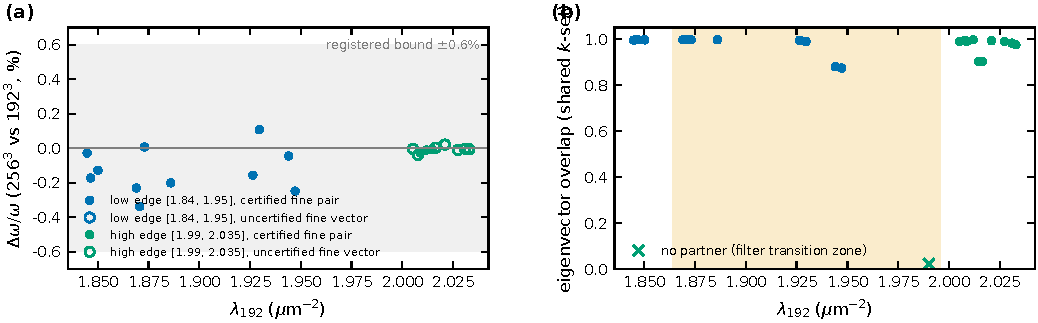
\includegraphics[width=\textwidth]{figS_crossgrid}
\caption{I6: (a) $\Delta\omega/\omega$ between $256^3$ and $192^3$ per matched state; (b) overlaps.}
\label{figS_crossgrid}
\end{figure}

\subsection{The seam test}\label{sec:seam}
The gap window $[1.855,2.000]$ was re-solved at $192^3$ on the periodically wrapped structure twice: $m=30$ (20.0~h; 7 converged pairs, 1 in-window unconverged at 1.9095) and $m=48$ (4 of 8 requested polish outers, stopped on a two-outer plateau; the same 7 pairs, agreeing with the first to $4.8\times10^{-5}$, exactly the normalization correction that the second run had built in; 2 unconverged at 1.8902 and 1.9534 with residuals $6\times10^{-2}$ throughout). Identity between the montage-convention and periodic states is decided by eigenvector overlap $>0.5$ in the shared plane-wave basis (Fig.~\ref{figS_periodic}), not by a $\lambda$ window (a $2\times10^{-3}$ window mis-called four persisting states because the physical shift is larger). Results: all six bulk in-gap states persist with overlaps $0.952$--$0.9997$ and $\Delta\lambda=-0.0007$ to $-0.0034$, every shift negative as required when the missing dielectric is added ($1.8690\to1.8683$, $1.8860\to1.8853$, $1.9264\to1.9242$, $1.9441\to1.9407$, $1.9738\to1.9708$, $1.9901\to1.9879$). Three seam-flagged states have no partner (best overlaps 0.006, 0.131, 0.090; total overlap budgets $\sum_j|\langle m|p_j\rangle|^2$ of $10^{-4}$, $0.020$, $0.009$). The fourth, 1.9472, has best overlap 0.30 and budget 0.097, $5$--$1000\times$ the others: periodic state 1.9407 has 0.9969 of its weight inside span\{1.9441, 1.9472\}, and the I2 audit of the periodic solve finds $+2.04\pm0.42$ states missing in the interval containing it. Since the same two-dimensional-subspace argument is used to accept the 192/256 pairing of this very pair (overlaps 0.879/0.873, combined 0.996/0.993), it cannot be rejected here: 1.9472 is \textbf{undetermined}. The one periodic state without an in-gap partner, 1.9839, is the montage state 2.0088 pulled into the gap by the added dielectric ($\Delta\lambda=-0.0248$, overlap 0.915); all seven periodic states have a montage partner above the rule. In-gap count after the fix: $10\to7$. Negative half of the verdict weakened: the periodic solve is incomplete, so ``no partner found'' is not ``vanished''. The seam-free re-solve's localization is in Table~\ref{tab:periodic}.

\begin{table}
\caption{Localization of the seven certified states of the seam-free re-solve ($m=48$).}
\label{tab:periodic}
\begin{tabular}{@{}lrrrrr@{}}
\hline\hline
$\lambda$ ($\umi$) & $p$ (\%) & $\xi$ ($\mu$m) & $r^2$ & $f_2$ (\%) & montage partner \\ \hline
1.8682 & 0.071 & 1.83 & 0.995 & 2.6 & 1.8690 \\
1.8852 & 0.034 & 1.78 & 0.992 & 2.8 & 1.8860 \\
1.9241 & 0.046 & 1.87 & 0.985 & 2.0 & 1.9264 \\
1.9406 & 0.500 & 2.24 & 0.988 & 4.2 & 1.9441 (extended in the montage run; resolved here) \\
1.9707 & 0.328 & 2.12 & 0.997 & 10.3 & 1.9738 \\
1.9839 & 0.587 & 2.55 & 0.994 & 13.1 & 2.0088 (pulled in from above) \\
1.9878 & 0.321 & 2.63 & 0.986 & 3.7 & 1.9901 \\
\hline\hline
\end{tabular}
\end{table}
\begin{figure}
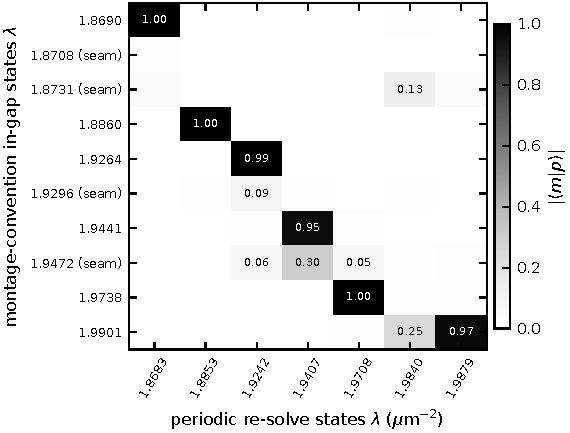
\includegraphics[width=0.6\textwidth]{figS_periodic}
\caption{Seam test: $|\langle m|p\rangle|$ between the ten montage-convention in-gap states (rows) and the seven periodic-solve states (columns), $m=30$ run.}
\label{figS_periodic}
\end{figure}

\section{Localization methodology}\label{sec:loc}
Per mode, from $u(\bm r)=\varepsilon|\bm E|^2$ on the $G^3$ grid (\texttt{eigenfns/localization.py}): participation ratio ${\rm PR}=(\sum u)^2/\sum u^2$ (voxels), participation fraction $p={\rm PR}/G^3$, participation volume $V_p={\rm PR}\,\delta x^3$ and radius $r_p=(3V_p/4\pi)^{1/3}$. Envelope decay length: azimuthal average of $u$ in 48 radial bins of minimum-image distance from the peak voxel up to $L/2$; least-squares line through $\ln u(r)$ over $[0.10,0.95]\,L/2$; $u\propto e^{-2r/\xi}$, so slope $=-2/\xi$. A fit is flagged \emph{unresolved} (lower bound only, never ``extended, $\xi=X$'') if $\xi\ge L/2$, if the profile decays by $<1$ decade over the range, or if $r^2<0.7$ (non-exponential shape); thresholds pre-registered. $N=10^4$: 121/133 resolved; the 12 unresolved all fail $r^2\ge0.7$, one also exceeds the ceiling. $N=1000$ circular: 42/210 resolved (141 above the $5.72\um$ ceiling, 77 fail $r^2$, overlapping); elliptical: 30/210.

\emph{Fit-range sensitivity.} Refitting over $[0.10,0.60]\,L/2$ changes $\xi$ by a median $|\Delta\xi|/\xi=30\%$ over the 121 resolved $N=10^4$ modes (compact modes, $p<0.2\%$: median ratio 0.75, range 0.49--1.16; extended, $p>1\%$: 0.66, range 0.48--1.64; Fig.~\ref{figS_fitrange}); far radial bins of extended modes catch other hot spots. Medians by spectral bin (resolved modes): $[1.757,1.80]$ 5.00, $[1.80,1.85]$ 3.01, $[1.85,1.864]$ 2.08, bracket 2.09, $[1.996,2.02]$ 2.79, $[2.02,2.07]$ 4.75, $[2.07,2.117]$ $6.11\um$; with the short range 3.64, 2.32, 1.72, 1.76, 2.05, 3.66, $3.79\um$. Window-end/near-edge contrasts: $\xi$ $1.7\times$ (below) and $2.2\times$ (above) with the full range, $1.8\times$/$1.6\times$ with the short range; $r_p$ $1.8\times$/$1.7\times$ ($r_p$ by bin: 2.65, 1.49, 1.15, 1.35, 3.12, 4.13, $5.43\um$); median $p$ by bin 0.52, 0.09, 0.04, 0.07, 0.85, 2.0, 4.5\%. Hot-spot spacing is flat at $\sim1\um$ (the rod scale) across all modes while $\xi$ varies $7\times$, so $\xi$ is not measuring hot-spot spacing. \emph{I8} (cross-solver $\xi$ agreement, $\le0.1\%$) shows the pipeline is deterministic, not that the estimator is accurate: both solvers hand it the same field to $\sim10^{-7}$.

\begin{figure}
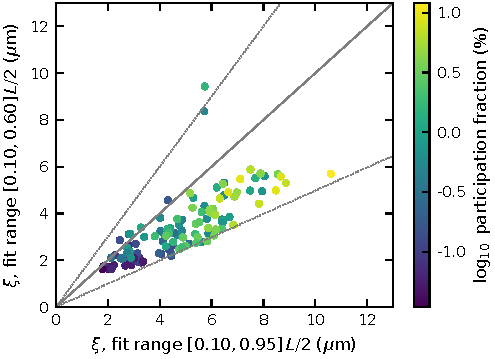
\includegraphics[width=0.6\textwidth]{figS_fitrange}
\caption{Fit-range sensitivity of $\xi$ for the 121 resolved $N=10^4$ modes; dotted lines at $0.5\times$ and $1.5\times$.}
\label{figS_fitrange}
\end{figure}

\section{Level statistics}
Adjacent-gap ratio $r_n=\min(s_n,s_{n-1})/\max(s_n,s_{n-1})$~\cite{Oganesyan2007}; surmises $P_{\rm P}(r)=2/(1+r)^2$ and $P_{\rm GOE}(r)=\frac{27}{8}(r+r^2)/(1+r+r^2)^{5/2}$, $\langle r\rangle_{\rm P}=2\ln2-1=0.3863$, $\langle r\rangle_{\rm GOE}=0.5307$ (large-$N$; the $3\times3$ surmise gives 0.5359)~\cite{Atas2013}. Bootstrap standard errors (20\,000 resamples). Bands and results (Table~\ref{tab:r}, Fig.~\ref{figS_levelstats}). Spacing distributions after local unfolding (9-level running mean) are shown for completeness; the ratio statistic is the one used. No pair of the 133 $N=10^4$ levels is closer than 5\% of the local spacing (Poisson expects 4.9\%, GOE 0.4\%); 1.8\% / 1.0\% of the 611 elliptical/circular $N=1000$ spacings are, reflecting accidental near-degeneracies that gate G4 resolved as subspaces. Log-likelihood ratios GOE vs Poisson from the surmises are strongly in favour of GOE for every band with $\ge40$ levels ($\ge27$ nats) and marginal for the 12-level near-edge band ($-1.5$... see \texttt{report/tables/levelstats.json}). The 7 states of the periodic re-solve are too few for any statistic. A Thouless-type sensitivity (twisted boundary conditions or $dE/dk$) would need re-solves at $k\ne\Gamma$ and is not available.

\begin{table}
\caption{Adjacent-gap ratios (bootstrap s.e.). Poisson 0.386, GOE 0.531.}
\label{tab:r}
\begin{tabular}{@{}lllrl@{}}
\hline\hline
spectrum & band & $\lambda$ range & levels & $\langle r\rangle$ \\ \hline
$N=10^4$ & below, extended & $<1.816$ & 51 & $0.528\pm0.038$ \\
$N=10^4$ & below, near edge & $1.821$--$1.850$ & 12 & $0.357\pm0.073$ \\
$N=10^4$ & in bracket (all ten) & $1.869$--$1.990$ & 10 & $0.314\pm0.081$ \\
$N=10^4$ & above, near edge & $2.005$--$2.050$ & 18 & $0.559\pm0.047$ \\
$N=10^4$ & above, extended & $>2.051$ & 42 & $0.528\pm0.041$ \\
$N=10^4$ & below bracket (all) & $<1.864$ & 63 & $0.498\pm0.035$ \\
$N=10^4$ & above bracket (all) & $>1.996$ & 60 & $0.541\pm0.032$ \\
$N=10^4$ & outside bracket, pooled $r$ & & 119 $r$ & $0.519\pm0.024$ \\
$N=10^4$ & all & & 133 & $0.501\pm0.023$ \\
$N=10^3$ ell. & bands 3--200 & & 198 & $0.486\pm0.019$ \\
$N=10^3$ ell. & bands 201--400 & & 200 & $0.495\pm0.019$ \\
$N=10^3$ ell. & bands 401--500 & & 100 & $0.526\pm0.026$ \\
$N=10^3$ ell. & bands 501--600 & & 100 & $0.542\pm0.026$ \\
$N=10^3$ ell. & all 611 & & 611 & $0.508\pm0.010$ \\
$N=10^3$ circ. & bands 401--500 & & 100 & $0.516\pm0.028$ \\
$N=10^3$ circ. & bands 501--600 & & 100 & $0.560\pm0.026$ \\
$N=10^3$ circ. & all 611 & & 611 & $0.533\pm0.011$ \\
\hline\hline
\end{tabular}
\end{table}
\begin{figure}
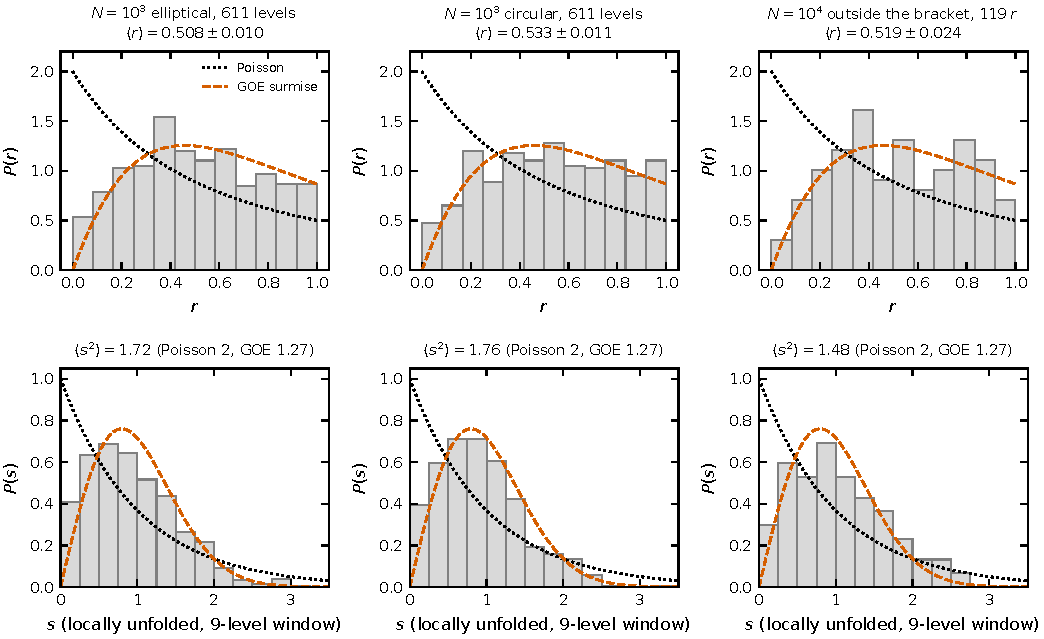
\includegraphics[width=\textwidth]{figS_levelstats}
\caption{$P(r)$ (top) and locally unfolded $P(s)$ (bottom) for the two $N=1000$ spectra and the $N=10^4$ levels outside the bracket, with the Poisson and GOE surmises.}
\label{figS_levelstats}
\end{figure}
\begin{figure}
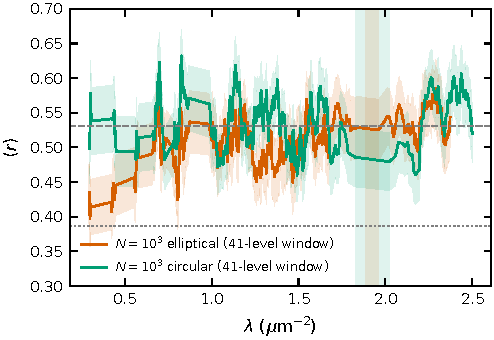
\includegraphics[width=0.6\textwidth]{figS_sliding_r_n1k}
\caption{Sliding 41-level $\langle r\rangle$ for the two $N=1000$ spectra; shaded: the gaps.}
\label{figS_slidingr}
\end{figure}

\section{Retracted and withdrawn claims}\label{sec:retracted}
The following statements were made during the project and are \emph{not} made in this paper. (1) \emph{Rare-region $z$-test} (retracted, round 4): the energy-weighted local filling fraction of the five candidates, $z$-scored against the $\xi$-coarse-grained field, gave $|z|=0.57$ vs $0.27$ for bulk controls. The controls were the most extended modes of the window ($p=0.7$--$12\%$) against the most compact candidates ($p=0.03$--$0.3\%$), a $36\times$ median volume difference, and energy-weighting a coarse-grained field is a shrinkage estimator, so the ratio was manufactured; against an extent-matched translation null $|z|/\sigma_{\rm null}$ is 2.77 for the candidates vs 7.19 for the controls ($p=0.999$ in the claimed direction). Only the finite-size statistics argument (matched local distributions; $10\times$ the draws; $P(\text{empty }N=1000\text{ gap})=0.61$) survives. (2) \emph{``The resolution confound is closed''} (withdrawn, round 4): the 99.98\% power retention of $256^3$ modes inside the $192^3$ $k$-set is saturated---a $96^3$ cube retains 99.8\% and the statistic is flat (99.975--99.984\%) across all 14 modes---and it measures band-limiting of $E$, not of $\varepsilon$. The I6 gate passes on its per-band criterion; that is all that is claimed. (3) \emph{``All four seam states vanished''}: 1.9472 is undetermined (Sec.~\ref{sec:seam}), and the periodic solve is incomplete. (4) \emph{Uncorrected eigenvalues} and every figure derived from them (I1 at $2.8\times10^{-5}$; proj$^2>1$). (5) \emph{KPM/eigensolver in-gap agreement as evidence against an artefact} ($11.18\pm0.58$ vs 10): KPM consumes the same rasterized $\varepsilon$ and sees the same seam; it rules out an eigensolver artefact only, and carries a $+1$ bias. (6) \emph{``$S_{\rm below}$ 69 predicted vs 69 found''} as a validation: with the $+7.7$ bias model the prediction is $\approx65$; the agreement was a coincidence. (7) The extended in-gap state 1.9441 was briefly listed as a localized candidate ($\xi=13.0\um>L/2$, $r^2=0.33$). (8) Stale ranges in early drafts (``$\xi=1.8$--$2.1\um$, $p=0.03$--$0.09\%$'', ``119 of 130 resolved'') superseded by 1.80--2.51, 0.034--0.33\%, 121 of 133.

\section{Honest limitations (full list)}
\begin{enumerate}
\item Gap-edge frequencies are rasterization-limited: 0.27\% non-monotone spread at $N=1000$ ($64^3/96^3/128^3$); the gap width is non-monotone (2.35/1.93/2.08\%); on the MPB-interpolated $64^3$ grid the elliptical 500|501 spacing is 0.60\% with the largest spacing at 501|502. Sub-percent gap-edge frequencies are not claimed at $192^3$ (7.8 vox/$\mu$m), where the 192/256 shifts are $\le0.34\%$.
\item Binary voxels (no subpixel smoothing) by design, for fidelity to the reference montage; a smoothed-$\varepsilon$ convention would be a different calculation.
\item The montage-convention rasterizer carries the boundary seam (11--13\% shell deficit) on all grids; the $N=1000$ windows contain modes with shell enhancement up to $4\times$; only the $N=10^4$ gap window was re-solved seam-free, and that re-solve is incomplete ($+2.0\pm0.4$ missed in its sub-interval; two solves left different states unconverged).
\item Completeness is certified on the sub-interval $[1.9063,1.9606]$ only; the full-window estimator is biased and the KPM population comparison is not a count.
\item I3 fails: the merged 133-mode set has cross-slice Gram deviations up to $4.9\times10^{-4}$; mechanism open.
\item $\xi$ is bounded by $L/2$, fit-range dependent at the 30\% level, and validated only for pipeline determinism (I8), not as an absolute estimator; 168/210 $N=1000$ modes are ceiling-limited.
\item One disorder realization per size; two sizes; no transport; no $k\ne\Gamma$ data (G1 not run).
\item fp32 device arithmetic with fp64 Rayleigh--Ritz; the normalization bug shows how such pipelines fail silently.
\item G4 was scope-limited to the lowest 30 bands; window degeneracies are certified only indirectly (parity $3.5\times10^{-5}$, Gram $1.2\times10^{-5}$).
\item Absolute $N=10^4$ band indices carry $\pm13$ (stochastic) and a $\approx-4.5$ Jackson bias; the $\pm2$ convention ambiguity against the original montage remains.
\item The 5.5~h $N=1000$ production missed its 4~h target; the I6 high-edge anchor certified only 3 of 11 pairs; the $160^3$ leg is edge-truncated; the first $256^3$ high-edge attempt (9.1~h) produced nothing.
\item ``No published 3-D supercell interior Maxwell eigensolver on GPU was found'' is stated as ``none found'', not as a first.
\end{enumerate}

\section{Tables}
Table~\ref{tab:states} lists all 133 certified $N=10^4$ states. The 210-row $N=1000$ window tables (both decorations) and all 611-band spectra are in the repository as \texttt{report/tables/states\_n1k\_\{ell,circ\}.csv} and \texttt{spectrum\_n1k\_\{ell,circ\}.csv}; Table~\ref{tab:edge_circ} shows the circular-decoration bands around the gap.

\begin{table}
\caption{$N=1000$, circular decoration, bands 494--507 at $128^3$ ($^{\rm u}$ = unresolved fit, lower bound).}
\label{tab:edge_circ}
\begin{tabular}{@{}rrrrrrl@{}}
\hline\hline
 band & $\lambda$ ($\mu$m$^{-2}$) & $\nu$ & $p$ (\%) & $V_p$ ($\mu$m$^3$) & $\xi$ ($\mu$m) & $r^2$ \\
\hline
 494 & 1.75286 & 0.4821 & 2.74 & 41.1 & 2.58 & 0.87 \\
 495 & 1.76650 & 0.4840 & 2.86 & 42.9 & 3.96$^\mathrm{u}$ & 0.61 \\
 496 & 1.76737 & 0.4841 & 3.91 & 58.5 & 4.82$^\mathrm{u}$ & 0.65 \\
 497 & 1.77580 & 0.4853 & 2.96 & 44.4 & 3.52$^\mathrm{u}$ & 0.68 \\
 498 & 1.77759 & 0.4855 & 1.33 & 19.9 & 2.94 & 0.84 \\
 499 & 1.78550 & 0.4866 & 0.59 & 8.8 & 1.73 & 0.94 \\
 500 & 1.82759 & 0.4923 & 0.42 & 6.2 & 1.47 & 0.97 \\
 501 & 2.02249 & 0.5179 & 3.86 & 57.8 & 2.30 & 0.95 \\
 502 & 2.05698 & 0.5223 & 10.82 & 162.0 & 4.14 & 0.96 \\
 503 & 2.07574 & 0.5246 & 13.24 & 198.2 & 3.41 & 0.96 \\
 504 & 2.10055 & 0.5278 & 11.25 & 168.4 & 3.50 & 0.88 \\
 505 & 2.11251 & 0.5293 & 19.80 & 296.4 & 12.70$^\mathrm{u}$ & 0.89 \\
 506 & 2.12920 & 0.5314 & 21.00 & 314.4 & 4.72$^\mathrm{u}$ & 0.93 \\
 507 & 2.13615 & 0.5322 & 22.23 & 332.8 & 4.73$^\mathrm{u}$ & 0.96 \\
\hline\hline
\end{tabular}

\end{table}
\begin{table}
\caption{$N=1000$, elliptical decoration, bands 494--507 at $128^3$.}
\label{tab:edge_ell}
\begin{tabular}{@{}rrrrrrl@{}}
\hline\hline
 band & $\lambda$ ($\mu$m$^{-2}$) & $\nu$ & $p$ (\%) & $V_p$ ($\mu$m$^3$) & $\xi$ ($\mu$m) & $r^2$ \\
\hline
 494 & 1.79589 & 0.4880 & 2.31 & 34.6 & 2.58 & 0.93 \\
 495 & 1.80177 & 0.4888 & 3.35 & 50.1 & 3.07 & 0.75 \\
 496 & 1.80684 & 0.4895 & 1.54 & 23.0 & 2.18 & 0.90 \\
 497 & 1.81992 & 0.4913 & 6.06 & 90.7 & 6.43$^\mathrm{u}$ & 0.50 \\
 498 & 1.82787 & 0.4923 & 4.48 & 67.1 & 4.92 & 0.73 \\
 499 & 1.84065 & 0.4940 & 0.86 & 12.8 & 2.05 & 0.92 \\
 500 & 1.88296 & 0.4997 & 0.81 & 12.2 & 1.82 & 0.97 \\
 501 & 1.96277 & 0.5102 & 7.82 & 117.1 & 2.92 & 0.99 \\
 502 & 1.98657 & 0.5132 & 7.19 & 107.7 & 2.36 & 0.99 \\
 503 & 2.01179 & 0.5165 & 12.11 & 181.3 & 3.50 & 0.99 \\
 504 & 2.02106 & 0.5177 & 17.28 & 258.8 & 4.29$^\mathrm{u}$ & 0.97 \\
 505 & 2.04004 & 0.5201 & 16.44 & 246.1 & 5.53$^\mathrm{u}$ & 0.79 \\
 506 & 2.04605 & 0.5209 & 18.03 & 269.9 & 6.19$^\mathrm{u}$ & 0.96 \\
 507 & 2.05624 & 0.5222 & 9.63 & 144.2 & 3.08 & 0.98 \\
\hline\hline
\end{tabular}

\end{table}

\begin{longtable}{@{}rrllllllllll@{}}
\caption{All 133 residual-certified $N=10^4$ eigenstates (corrected $\lambda=\lambda_\mathrm{raw}/\|x\|^2$). $\nu=\sqrt{\lambda}\,a/2\pi$ with $a=2.288\,\mu$m. Residuals are the reported (raw-$\lambda$) values. $p$ is the participation fraction; $\xi$ the envelope decay length (`u' = unresolved: lower bound only; ceiling $L/2=12.32\,\mu$m); $f_2$ the energy fraction in the outer 2-voxel shell (volume fraction 6.1\%). Class: g = inside the nominal bracket [1.864, 1.996]; seam = boundary-seam artefact (seam* = undetermined, see text); ext.\ = extended in-gap mode. Periodic: best-overlap partner in the seam-free re-solve (in-gap states only).}\label{tab:states}\\
\hline\hline
 \# & tile & $\lambda$ ($\mu$m$^{-2}$) & $\nu$ & res. & $p$ (\%) & $\xi$ ($\mu$m) & $r^2$ & $f_2$ (\%) & slice & class & periodic \\
\hline
\endfirsthead
\hline
 \# & tile & $\lambda$ & $\nu$ & res. & $p$ (\%) & $\xi$ & $r^2$ & $f_2$ (\%) & slice & class & periodic \\
\hline
\endhead
\hline
\endfoot
\hline\hline
\endlastfoot
 0 & 4942 & 1.75705 & 0.4827 & $6.1\times10^{-5}$ & 1.294 & 6.20 & 0.90 & 5.8 & Sbelow &  &  \\
 1 & 4943 & 1.75739 & 0.4827 & $6.2\times10^{-5}$ & 0.899 & 5.30 & 0.95 & 6.4 & Sbelow &  &  \\
 2 & 4944 & 1.75835 & 0.4829 & $6.1\times10^{-5}$ & 0.717 & 7.95 & 0.73 & 8.8 & Sbelow &  &  \\
 3 & 4945 & 1.75917 & 0.4830 & $6.1\times10^{-5}$ & 1.286 & 7.87u & 0.62 & 5.8 & Sbelow &  &  \\
 4 & 4946 & 1.76006 & 0.4831 & $6.1\times10^{-5}$ & 1.358 & 7.69 & 0.84 & 7.1 & Sbelow &  &  \\
 5 & 4947 & 1.76054 & 0.4832 & $6.0\times10^{-5}$ & 1.073 & 7.49 & 0.83 & 3.0 & Sbelow &  &  \\
 6 & 4948 & 1.76138 & 0.4833 & $6.1\times10^{-5}$ & 0.608 & 6.40 & 0.78 & 4.8 & Sbelow &  &  \\
 7 & 4949 & 1.76157 & 0.4833 & $6.0\times10^{-5}$ & 0.667 & 4.75 & 0.89 & 7.5 & Sbelow &  &  \\
 8 & 4950 & 1.76246 & 0.4834 & $6.0\times10^{-5}$ & 0.567 & 6.48 & 0.85 & 3.6 & Sbelow &  &  \\
 9 & 4951 & 1.76369 & 0.4836 & $6.0\times10^{-5}$ & 0.238 & 4.02 & 0.94 & 6.0 & Sbelow &  &  \\
 10 & 4952 & 1.76504 & 0.4838 & $6.2\times10^{-5}$ & 0.694 & 8.04 & 0.77 & 5.5 & Sbelow &  &  \\
 11 & 4953 & 1.76516 & 0.4838 & $6.2\times10^{-5}$ & 1.014 & 6.44 & 0.78 & 9.2 & Sbelow &  &  \\
 12 & 4954 & 1.76540 & 0.4838 & $6.0\times10^{-5}$ & 0.754 & 6.42 & 0.76 & 8.2 & Sbelow &  &  \\
 13 & 4955 & 1.76571 & 0.4839 & $6.1\times10^{-5}$ & 0.619 & 5.81 & 0.81 & 11.0 & Sbelow &  &  \\
 14 & 4956 & 1.76656 & 0.4840 & $6.1\times10^{-5}$ & 0.879 & 6.69 & 0.75 & 6.4 & Sbelow &  &  \\
 15 & 4957 & 1.76754 & 0.4841 & $6.1\times10^{-5}$ & 0.527 & 4.12 & 0.95 & 6.0 & Sbelow &  &  \\
 16 & 4958 & 1.76810 & 0.4842 & $5.9\times10^{-5}$ & 0.536 & 5.87 & 0.73 & 7.7 & Sbelow &  &  \\
 17 & 4959 & 1.76892 & 0.4843 & $6.2\times10^{-5}$ & 0.389 & 4.03 & 0.92 & 10.2 & Sbelow &  &  \\
 18 & 4960 & 1.76910 & 0.4843 & $6.2\times10^{-5}$ & 0.482 & 4.86 & 0.84 & 10.0 & Sbelow &  &  \\
 19 & 4961 & 1.77082 & 0.4846 & $5.9\times10^{-5}$ & 0.234 & 4.11 & 0.89 & 2.5 & Sbelow &  &  \\
 20 & 4962 & 1.77127 & 0.4846 & $5.9\times10^{-5}$ & 0.481 & 8.66u & 0.51 & 4.9 & Sbelow &  &  \\
 21 & 4963 & 1.77420 & 0.4850 & $5.9\times10^{-5}$ & 0.522 & 5.71 & 0.91 & 13.4 & Sbelow &  &  \\
 22 & 4964 & 1.77656 & 0.4854 & $5.9\times10^{-5}$ & 0.594 & 5.73 & 0.86 & 4.2 & Sbelow &  &  \\
 23 & 4965 & 1.77677 & 0.4854 & $6.0\times10^{-5}$ & 0.453 & 6.49 & 0.82 & 5.5 & Sbelow &  &  \\
 24 & 4966 & 1.77858 & 0.4856 & $5.9\times10^{-5}$ & 0.143 & 4.07 & 0.79 & 1.9 & Sbelow &  &  \\
 25 & 4967 & 1.77929 & 0.4857 & $5.9\times10^{-5}$ & 0.153 & 4.45 & 0.71 & 0.8 & Sbelow &  &  \\
 26 & 4968 & 1.78053 & 0.4859 & $6.1\times10^{-5}$ & 0.562 & 4.69 & 0.88 & 1.2 & Sbelow &  &  \\
 27 & 4969 & 1.78157 & 0.4860 & $6.0\times10^{-5}$ & 0.577 & 4.00 & 0.98 & 11.5 & Sbelow &  &  \\
 28 & 4970 & 1.78291 & 0.4862 & $6.1\times10^{-5}$ & 0.534 & 5.63 & 0.71 & 8.4 & Sbelow &  &  \\
 29 & 4971 & 1.78511 & 0.4865 & $6.2\times10^{-5}$ & 0.105 & 4.51 & 0.78 & 1.4 & Sbelow &  &  \\
 30 & 4972 & 1.78599 & 0.4866 & $6.4\times10^{-5}$ & 0.064 & 2.69 & 0.95 & 0.7 & Sbelow &  &  \\
 31 & 4973 & 1.78791 & 0.4869 & $6.1\times10^{-5}$ & 0.172 & 4.32 & 0.88 & 11.2 & Sbelow &  &  \\
 32 & 4974 & 1.78938 & 0.4871 & $6.2\times10^{-5}$ & 0.466 & 4.86 & 0.92 & 6.4 & Sbelow &  &  \\
 33 & 4975 & 1.79004 & 0.4872 & $6.3\times10^{-5}$ & 0.279 & 5.13 & 0.79 & 3.1 & Sbelow &  &  \\
 34 & 4976 & 1.79097 & 0.4873 & $6.2\times10^{-5}$ & 0.136 & 3.07 & 0.97 & 3.4 & Sbelow &  &  \\
 35 & 4977 & 1.79460 & 0.4878 & $6.1\times10^{-5}$ & 0.071 & 3.22 & 0.90 & 6.2 & Sbelow &  &  \\
 36 & 4978 & 1.79596 & 0.4880 & $6.0\times10^{-5}$ & 0.293 & 2.81 & 0.98 & 16.8 & Sbelow &  &  \\
 37 & 4979 & 1.79713 & 0.4882 & $6.1\times10^{-5}$ & 0.465 & 8.57u & 0.56 & 13.0 & Sbelow &  &  \\
 38 & 4980 & 1.79765 & 0.4882 & $6.0\times10^{-5}$ & 0.359 & 4.56u & 0.68 & 19.2 & Sbelow &  &  \\
 39 & 4981 & 1.79793 & 0.4883 & $6.1\times10^{-5}$ & 0.347 & 6.14u & 0.62 & 17.9 & Sbelow &  &  \\
 40 & 4982 & 1.79885 & 0.4884 & $6.0\times10^{-5}$ & 0.220 & 3.97 & 0.80 & 3.9 & Sbelow &  &  \\
 41 & 4983 & 1.80001 & 0.4886 & $6.2\times10^{-5}$ & 0.122 & 3.01 & 0.91 & 5.3 & Sbelow &  &  \\
 42 & 4984 & 1.80045 & 0.4886 & $6.0\times10^{-5}$ & 0.261 & 4.54 & 0.86 & 3.7 & Sbelow &  &  \\
 43 & 4985 & 1.80290 & 0.4889 & $6.0\times10^{-5}$ & 0.221 & 4.44 & 0.75 & 8.2 & Sbelow &  &  \\
 44 & 4986 & 1.80362 & 0.4890 & $6.1\times10^{-5}$ & 0.230 & 2.70 & 0.93 & 16.3 & Sbelow &  &  \\
 45 & 4987 & 1.80435 & 0.4891 & $6.4\times10^{-5}$ & 0.149 & 4.36 & 0.77 & 4.3 & Sbelow &  &  \\
 46 & 4988 & 1.80530 & 0.4893 & $6.2\times10^{-5}$ & 0.097 & 3.04 & 0.91 & 3.5 & Sbelow &  &  \\
 47 & 4989 & 1.80639 & 0.4894 & $6.2\times10^{-5}$ & 0.053 & 2.90 & 0.85 & 0.4 & Sbelow &  &  \\
 48 & 4990 & 1.80754 & 0.4896 & $6.4\times10^{-5}$ & 0.207 & 3.06 & 0.94 & 27.9 & Sbelow &  &  \\
 49 & 4991 & 1.81234 & 0.4902 & $6.0\times10^{-5}$ & 0.059 & 2.24 & 0.98 & 0.5 & Sbelow &  &  \\
 50 & 4992 & 1.81592 & 0.4907 & $6.2\times10^{-5}$ & 0.093 & 2.28 & 0.98 & 1.6 & Sbelow &  &  \\
 51 & 4993 & 1.82084 & 0.4914 & $6.0\times10^{-5}$ & 0.081 & 3.06 & 0.91 & 24.8 & Sbelow &  &  \\
 52 & 4994 & 1.82172 & 0.4915 & $6.1\times10^{-5}$ & 0.080 & 3.28 & 0.86 & 15.1 & Sbelow &  &  \\
 53 & 4995 & 1.82277 & 0.4916 & $6.1\times10^{-5}$ & 0.109 & 3.20 & 0.88 & 2.2 & Sbelow &  &  \\
 54 & 4996 & 1.82312 & 0.4917 & $6.4\times10^{-5}$ & 0.055 & 2.68 & 0.91 & 4.4 & Sbelow &  &  \\
 55 & 4997 & 1.82437 & 0.4919 & $6.0\times10^{-5}$ & 0.053 & 3.36 & 0.85 & 2.7 & Sbelow &  &  \\
 56 & 4998 & 1.82960 & 0.4926 & $6.1\times10^{-5}$ & 0.057 & 2.87 & 0.93 & 6.0 & Sbelow &  &  \\
 57 & 4999 & 1.82983 & 0.4926 & $5.9\times10^{-5}$ & 0.139 & 3.14 & 0.95 & 1.5 & Sbelow &  &  \\
 58 & 5000 & 1.83504 & 0.4933 & $6.0\times10^{-5}$ & 0.078 & 2.80 & 0.95 & 18.5 & Sbelow &  &  \\
 59 & 5001 & 1.83796 & 0.4937 & $6.0\times10^{-5}$ & 0.137 & 2.46 & 0.97 & 18.3 & Sbelow &  &  \\
 60 & 5002 & 1.84478 & 0.4946 & $5.8\times10^{-5}$ & 0.066 & 2.03 & 0.98 & 0.7 & Sbelow &  &  \\
 61 & 5003 & 1.84662 & 0.4948 & $6.1\times10^{-5}$ & 0.039 & 1.98 & 0.97 & 5.0 & Sbelow &  &  \\
 62 & 5004 & 1.85015 & 0.4953 & $6.1\times10^{-5}$ & 0.042 & 2.08 & 0.97 & 5.6 & Sbelow &  &  \\
 63 & 5005 & 1.86898 & 0.4978 & $5.9\times10^{-5}$ & 0.072 & 1.91 & 0.99 & 2.7 & Sbelow & g (cand.) & 1.8683 (0.999) \\
 64 & 5006 & 1.87076 & 0.4981 & $5.9\times10^{-5}$ & 0.048 & 1.83 & 0.99 & 18.2 & Sbelow & seam & -- (0.006) \\
 65 & 5007 & 1.87308 & 0.4984 & $6.1\times10^{-5}$ & 0.093 & 1.91 & 0.99 & 23.6 & Sbelow & seam & -- (0.131) \\
 66 & 5008 & 1.88601 & 0.5001 & $6.0\times10^{-5}$ & 0.034 & 1.80 & 0.99 & 2.8 & Sbelow & g (cand.) & 1.8853 (1.000) \\
 67 & 5009 & 1.92641 & 0.5054 & $5.7\times10^{-5}$ & 0.046 & 2.09 & 0.97 & 2.5 & Sbelow & g (cand.) & 1.9242 (0.994) \\
 68 & 5010 & 1.92960 & 0.5058 & $6.3\times10^{-5}$ & 0.065 & 2.14 & 0.96 & 43.7 & Sbelow & seam & -- (0.090) \\
 69 & 5011 & 1.94405 & 0.5077 & $5.5\times10^{-5}$ & 0.558 & 12.97u & 0.32 & 8.1 & Sgap & ext. & 1.9407 (0.952) \\
 70 & 5012 & 1.94721 & 0.5081 & $5.6\times10^{-5}$ & 0.053 & 3.01 & 0.92 & 42.1 & Sgap & seam* & -- (0.301) \\
 71 & 5013 & 1.97381 & 0.5116 & $5.4\times10^{-5}$ & 0.329 & 2.13 & 1.00 & 10.5 & Sgap & g (cand.) & 1.9708 (0.997) \\
 72 & 5014 & 1.99012 & 0.5137 & $5.2\times10^{-5}$ & 0.290 & 2.51 & 0.98 & 3.0 & Sabove & g (cand.) & 1.9879 (0.968) \\
 73 & 5015 & 2.00521 & 0.5157 & $5.3\times10^{-5}$ & 0.339 & 2.56 & 0.96 & 0.7 & Sabove &  &  \\
 74 & 5016 & 2.00769 & 0.5160 & $5.1\times10^{-5}$ & 0.919 & 2.75 & 0.99 & 2.7 & Sabove &  &  \\
 75 & 5017 & 2.00879 & 0.5161 & $5.2\times10^{-5}$ & 0.789 & 2.84 & 0.95 & 12.4 & Sabove &  &  \\
 76 & 5018 & 2.01185 & 0.5165 & $5.3\times10^{-5}$ & 0.418 & 2.74 & 0.97 & 19.6 & Sabove &  &  \\
 77 & 5019 & 2.01468 & 0.5169 & $5.2\times10^{-5}$ & 1.145 & 5.49 & 0.77 & 1.6 & Sabove &  &  \\
 78 & 5020 & 2.01637 & 0.5171 & $5.1\times10^{-5}$ & 1.167 & 4.40 & 0.92 & 1.6 & Sabove &  &  \\
 79 & 5021 & 2.02093 & 0.5177 & $5.1\times10^{-5}$ & 0.789 & 3.40 & 0.99 & 14.7 & Sabove &  &  \\
 80 & 5022 & 2.02738 & 0.5185 & $5.3\times10^{-5}$ & 1.971 & 5.62 & 0.92 & 8.7 & Sabove &  &  \\
 81 & 5023 & 2.03088 & 0.5189 & $5.2\times10^{-5}$ & 1.605 & 5.74 & 0.94 & 16.0 & Sabove &  &  \\
 82 & 5024 & 2.03292 & 0.5192 & $5.1\times10^{-5}$ & 1.962 & 3.82 & 0.97 & 6.2 & Sabove &  &  \\
 83 & 5025 & 2.03675 & 0.5197 & $5.2\times10^{-5}$ & 2.057 & 4.68 & 0.97 & 5.0 & Sabove &  &  \\
 84 & 5026 & 2.03965 & 0.5201 & $5.2\times10^{-5}$ & 0.660 & 2.89 & 0.93 & 20.2 & Sabove &  &  \\
 85 & 5027 & 2.04057 & 0.5202 & $5.1\times10^{-5}$ & 0.717 & 2.87 & 0.99 & 0.6 & Sabove &  &  \\
 86 & 5028 & 2.04245 & 0.5204 & $5.1\times10^{-5}$ & 4.795 & 6.97 & 0.88 & 8.8 & Sabove &  &  \\
 87 & 5029 & 2.04526 & 0.5208 & $5.1\times10^{-5}$ & 1.161 & 3.28 & 0.98 & 1.7 & Sabove &  &  \\
 88 & 5030 & 2.04616 & 0.5209 & $5.3\times10^{-5}$ & 1.785 & 5.37 & 0.82 & 5.1 & Sabove &  &  \\
 89 & 5031 & 2.04712 & 0.5210 & $5.5\times10^{-5}$ & 3.580 & 8.55 & 0.83 & 3.7 & Sabove &  &  \\
 90 & 5032 & 2.04952 & 0.5213 & $5.3\times10^{-5}$ & 1.490 & 4.30 & 0.95 & 5.2 & Sabove &  &  \\
 91 & 5033 & 2.05075 & 0.5215 & $5.1\times10^{-5}$ & 2.789 & 4.75 & 0.78 & 4.6 & Sabove &  &  \\
 92 & 5034 & 2.05228 & 0.5217 & $5.2\times10^{-5}$ & 3.628 & 6.05 & 0.85 & 3.1 & Sabove &  &  \\
 93 & 5035 & 2.05373 & 0.5219 & $5.1\times10^{-5}$ & 4.267 & 7.89 & 0.92 & 5.1 & Sabove &  &  \\
 94 & 5036 & 2.05458 & 0.5220 & $5.1\times10^{-5}$ & 1.984 & 4.36 & 0.93 & 3.0 & Sabove &  &  \\
 95 & 5037 & 2.05686 & 0.5223 & $5.1\times10^{-5}$ & 1.148 & 4.23 & 0.87 & 9.3 & Sabove &  &  \\
 96 & 5038 & 2.05765 & 0.5224 & $5.1\times10^{-5}$ & 4.102 & 6.44 & 0.94 & 4.8 & Sabove &  &  \\
 97 & 5039 & 2.06035 & 0.5227 & $5.2\times10^{-5}$ & 2.365 & 6.40 & 0.79 & 1.9 & Sabove &  &  \\
 98 & 5040 & 2.06442 & 0.5232 & $5.2\times10^{-5}$ & 4.786 & 11.02u & 0.44 & 5.5 & Sabove &  &  \\
 99 & 5041 & 2.06639 & 0.5235 & $5.3\times10^{-5}$ & 2.997 & 5.39 & 0.91 & 4.5 & Sabove &  &  \\
 100 & 5042 & 2.06908 & 0.5238 & $5.4\times10^{-5}$ & 1.548 & 4.53 & 0.88 & 5.1 & Sabove &  &  \\
 101 & 5043 & 2.07022 & 0.5239 & $5.3\times10^{-5}$ & 3.201 & 5.46 & 0.81 & 4.6 & Sabove &  &  \\
 102 & 5044 & 2.07044 & 0.5240 & $5.3\times10^{-5}$ & 2.958 & 4.90 & 0.88 & 2.8 & Sabove &  &  \\
 103 & 5045 & 2.07270 & 0.5243 & $5.1\times10^{-5}$ & 2.800 & 4.24 & 0.94 & 5.7 & Sabove &  &  \\
 104 & 5046 & 2.07504 & 0.5246 & $5.2\times10^{-5}$ & 6.362 & 7.50 & 0.93 & 6.4 & Sabove &  &  \\
 105 & 5047 & 2.07622 & 0.5247 & $5.1\times10^{-5}$ & 3.655 & 7.65u & 0.68 & 4.2 & Sabove &  &  \\
 106 & 5048 & 2.07704 & 0.5248 & $5.2\times10^{-5}$ & 4.660 & 5.92 & 0.91 & 3.1 & Sabove &  &  \\
 107 & 5049 & 2.07867 & 0.5250 & $5.1\times10^{-5}$ & 6.107 & 6.84 & 0.78 & 5.4 & Sabove &  &  \\
 108 & 5050 & 2.08010 & 0.5252 & $5.2\times10^{-5}$ & 3.429 & 6.11 & 0.77 & 4.1 & Sabove &  &  \\
 109 & 5051 & 2.08059 & 0.5253 & $5.2\times10^{-5}$ & 4.452 & 5.96 & 0.92 & 5.2 & Sabove &  &  \\
 110 & 5052 & 2.08201 & 0.5254 & $5.1\times10^{-5}$ & 3.183 & 5.83 & 0.73 & 3.5 & Sabove &  &  \\
 111 & 5053 & 2.08464 & 0.5258 & $5.2\times10^{-5}$ & 2.789 & 5.01 & 0.79 & 2.9 & Sabove &  &  \\
 112 & 5054 & 2.08537 & 0.5259 & $5.2\times10^{-5}$ & 3.485 & 5.46u & 0.70 & 4.8 & Sabove &  &  \\
 113 & 5055 & 2.08721 & 0.5261 & $5.2\times10^{-5}$ & 3.900 & 7.63u & 0.53 & 4.3 & Sabove &  &  \\
 114 & 5056 & 2.08938 & 0.5264 & $5.2\times10^{-5}$ & 2.008 & 4.86 & 0.79 & 3.6 & Sabove &  &  \\
 115 & 5057 & 2.08980 & 0.5264 & $5.3\times10^{-5}$ & 2.390 & 5.40 & 0.75 & 3.2 & Sabove &  &  \\
 116 & 5058 & 2.09186 & 0.5267 & $5.2\times10^{-5}$ & 2.622 & 5.53 & 0.89 & 5.8 & Sabove &  &  \\
 117 & 5059 & 2.09342 & 0.5269 & $5.1\times10^{-5}$ & 7.178 & 7.83 & 0.80 & 4.5 & Sabove &  &  \\
 118 & 5060 & 2.09473 & 0.5270 & $5.1\times10^{-5}$ & 7.073 & 8.87 & 0.80 & 5.4 & Sabove &  &  \\
 119 & 5061 & 2.09679 & 0.5273 & $5.1\times10^{-5}$ & 8.666 & 8.67 & 0.88 & 6.1 & Sabove &  &  \\
 120 & 5062 & 2.09806 & 0.5275 & $5.2\times10^{-5}$ & 5.411 & 6.14 & 0.86 & 6.9 & Sabove &  &  \\
 121 & 5063 & 2.09911 & 0.5276 & $5.1\times10^{-5}$ & 9.304 & 10.91u & 0.68 & 7.4 & Sabove &  &  \\
 122 & 5064 & 2.09937 & 0.5276 & $5.2\times10^{-5}$ & 4.371 & 5.88 & 0.83 & 7.0 & Sabove &  &  \\
 123 & 5065 & 2.10012 & 0.5277 & $5.2\times10^{-5}$ & 5.239 & 6.88 & 0.88 & 6.3 & Sabove &  &  \\
 124 & 5066 & 2.10272 & 0.5280 & $5.2\times10^{-5}$ & 3.710 & 5.26 & 0.98 & 5.7 & Sabove &  &  \\
 125 & 5067 & 2.10484 & 0.5283 & $5.2\times10^{-5}$ & 4.503 & 5.17 & 0.99 & 2.7 & Sabove &  &  \\
 126 & 5068 & 2.10723 & 0.5286 & $5.1\times10^{-5}$ & 8.960 & 6.65 & 0.95 & 7.1 & Sabove &  &  \\
 127 & 5069 & 2.10743 & 0.5286 & $5.1\times10^{-5}$ & 7.584 & 8.75u & 0.66 & 7.0 & Sabove &  &  \\
 128 & 5070 & 2.10954 & 0.5289 & $5.2\times10^{-5}$ & 12.082 & 10.60 & 0.73 & 5.1 & Sabove &  &  \\
 129 & 5071 & 2.11240 & 0.5293 & $5.6\times10^{-5}$ & 6.958 & 6.32 & 0.90 & 3.1 & Sabove &  &  \\
 130 & 5072 & 2.11383 & 0.5294 & $8.7\times10^{-5}$ & 9.603 & 7.11 & 0.96 & 5.6 & Sabove &  &  \\
 131 & 5073 & 2.11503 & 0.5296 & $6.1\times10^{-5}$ & 3.770 & 6.16 & 0.81 & 3.4 & Sabove &  &  \\
 132 & 5074 & 2.11657 & 0.5298 & $6.2\times10^{-5}$ & 9.293 & 8.47 & 0.81 & 5.7 & Sabove &  &  \\
\end{longtable}


\section{Extended figures}
\begin{figure}
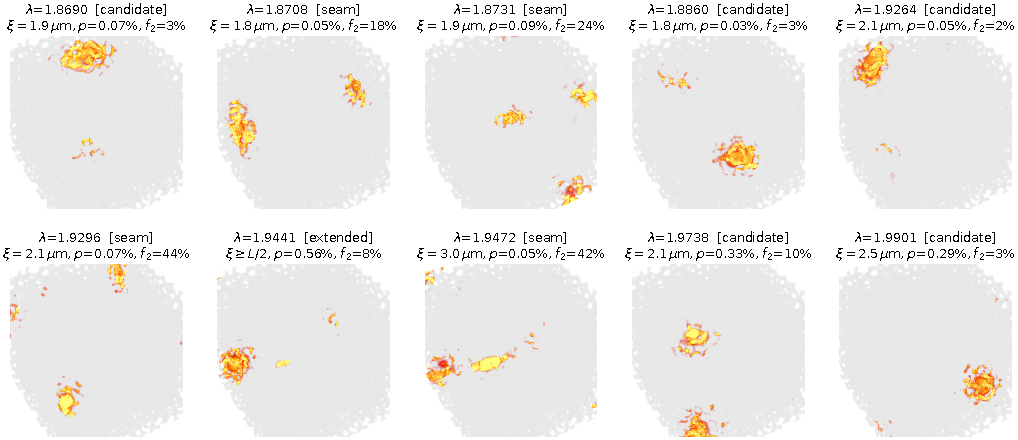
\includegraphics[width=\textwidth]{figS_ingap_tiles}
\caption{The ten certified $N=10^4$ states inside the nominal gap (montage-convention run), with class, $\xi$, $p$ and outer-shell energy fraction $f_2$.}
\label{figS_ingap}
\end{figure}
\begin{figure}
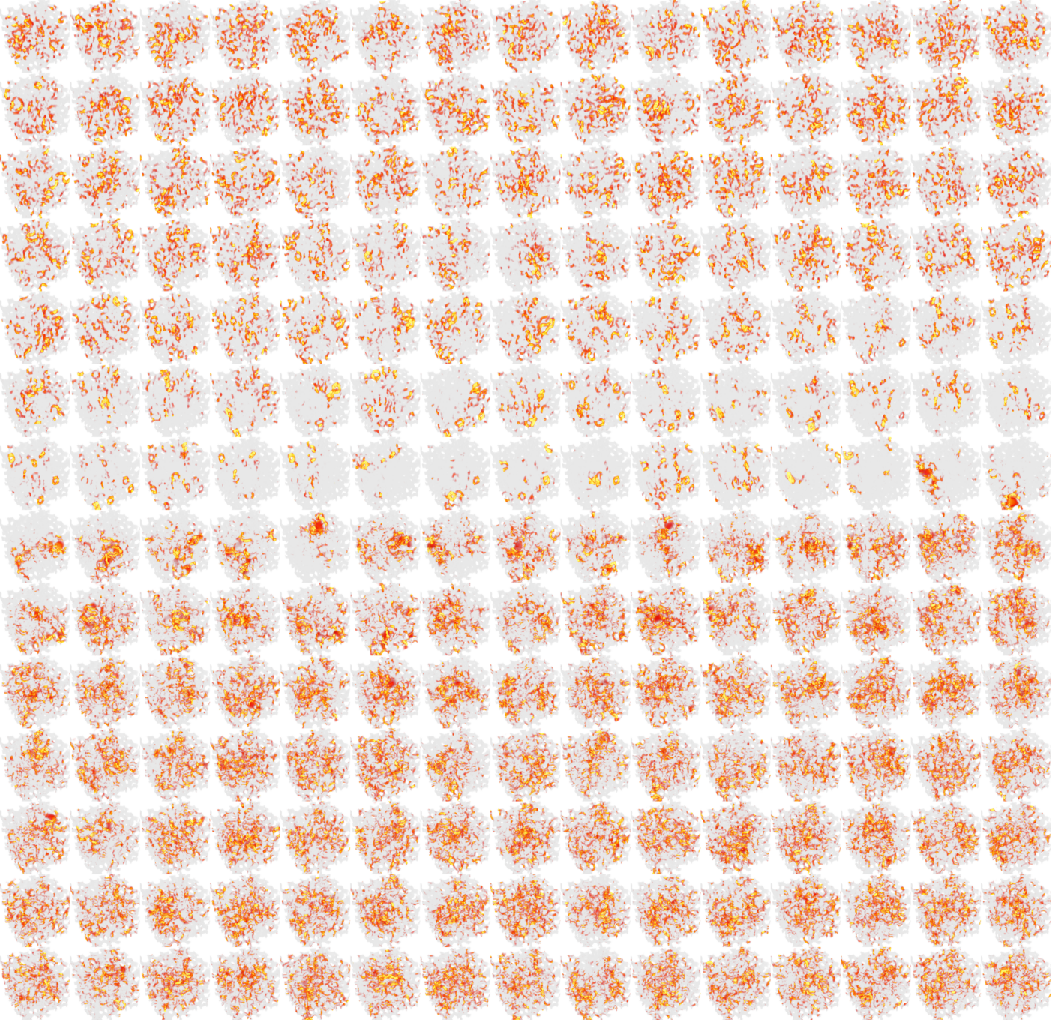
\includegraphics[width=\textwidth]{figS_montage_n1k_ell}
\caption{$N=1000$, elliptical decoration: the regenerated 210-tile montage of bands 398--607 (15 per row, row-major), $\varepsilon|\bm E|^2$ at $128^3$.}
\label{figS_montage_ell}
\end{figure}
\begin{figure}
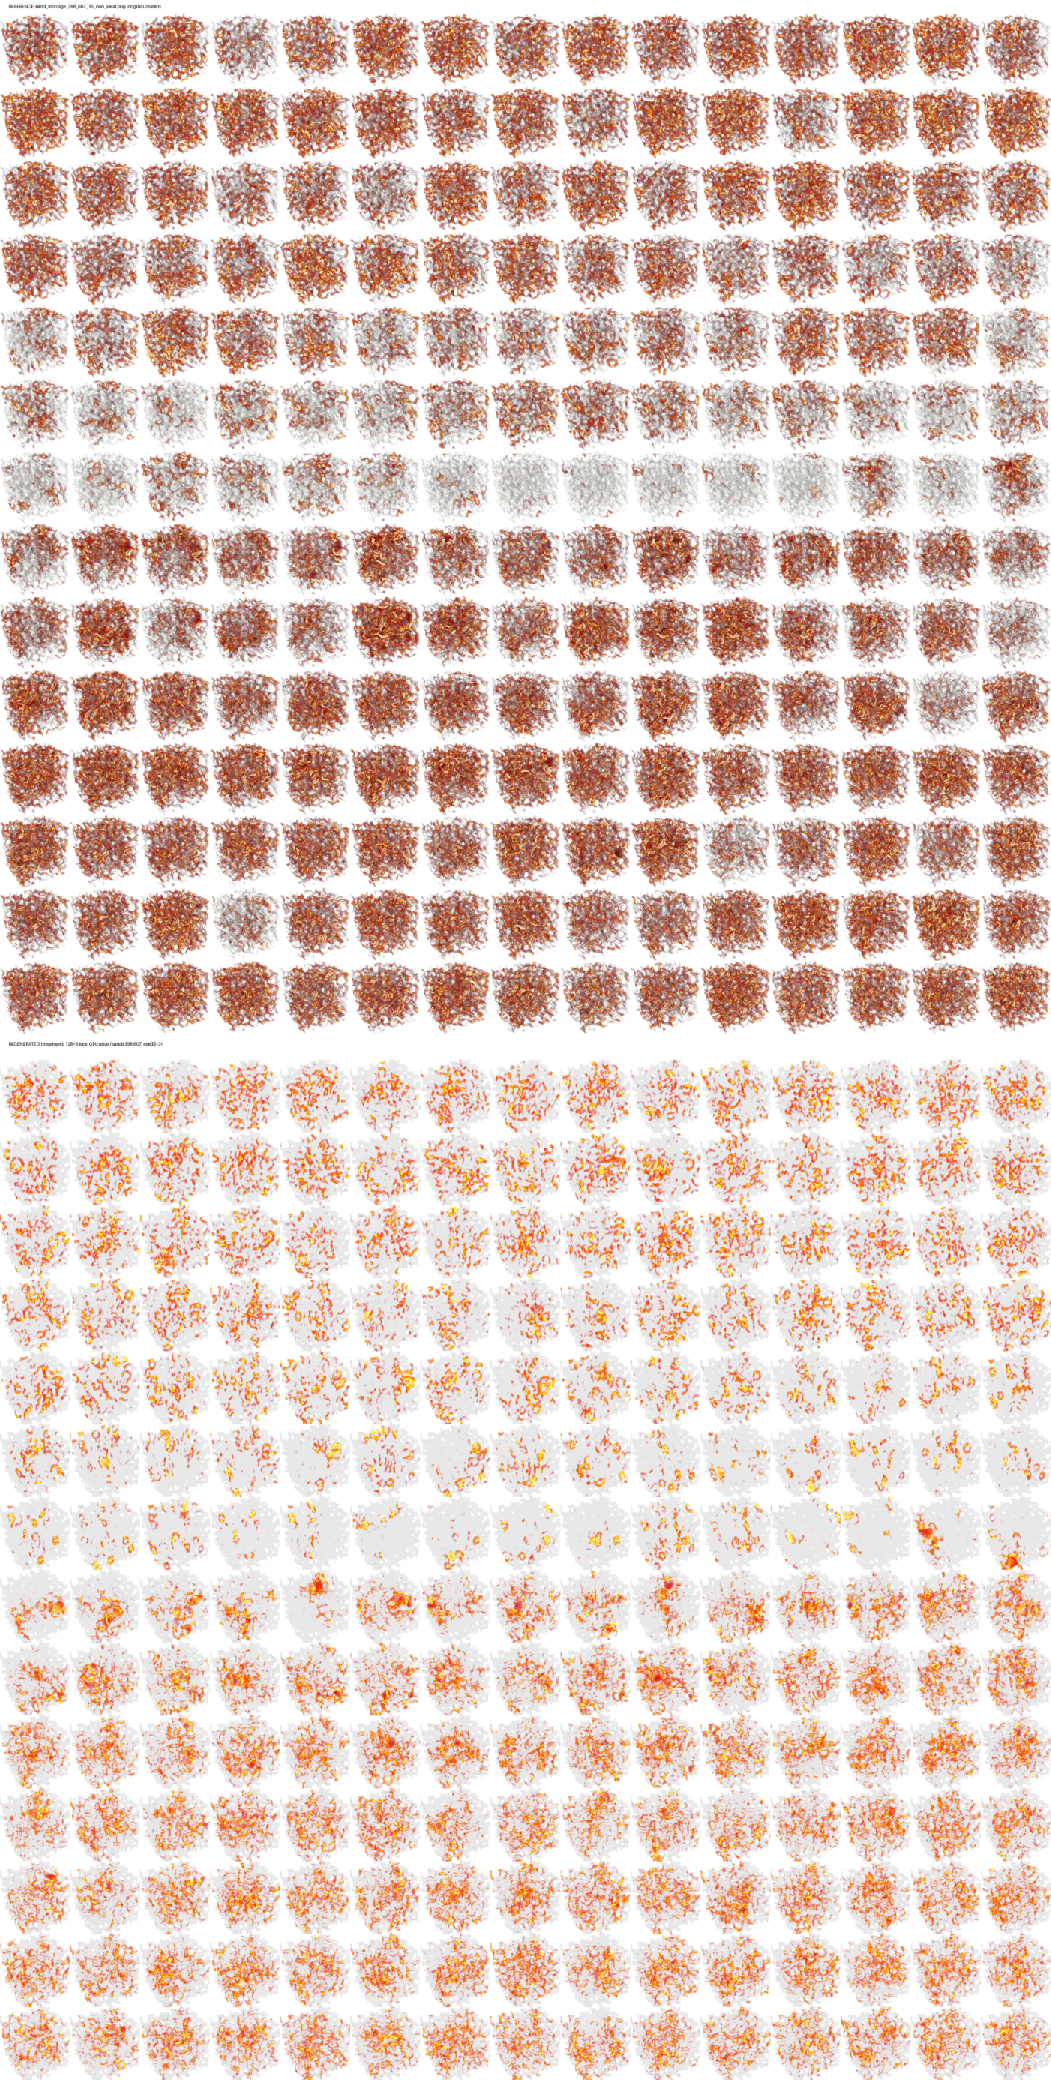
\includegraphics[width=0.75\textwidth]{figS_montage_sbs}
\caption{Left: the original cluster montage \texttt{band\_montage\_398\_607\_15\_non\_ideal.png}; right: our regeneration (same layout). The grey/bright row pattern (localized band-edge rows, extended deep-window rows) is reproduced tile for tile in character; the $\pm2$ labelling ambiguity is not resolved by this comparison.}
\label{figS_montage_sbs}
\end{figure}
\begin{figure}
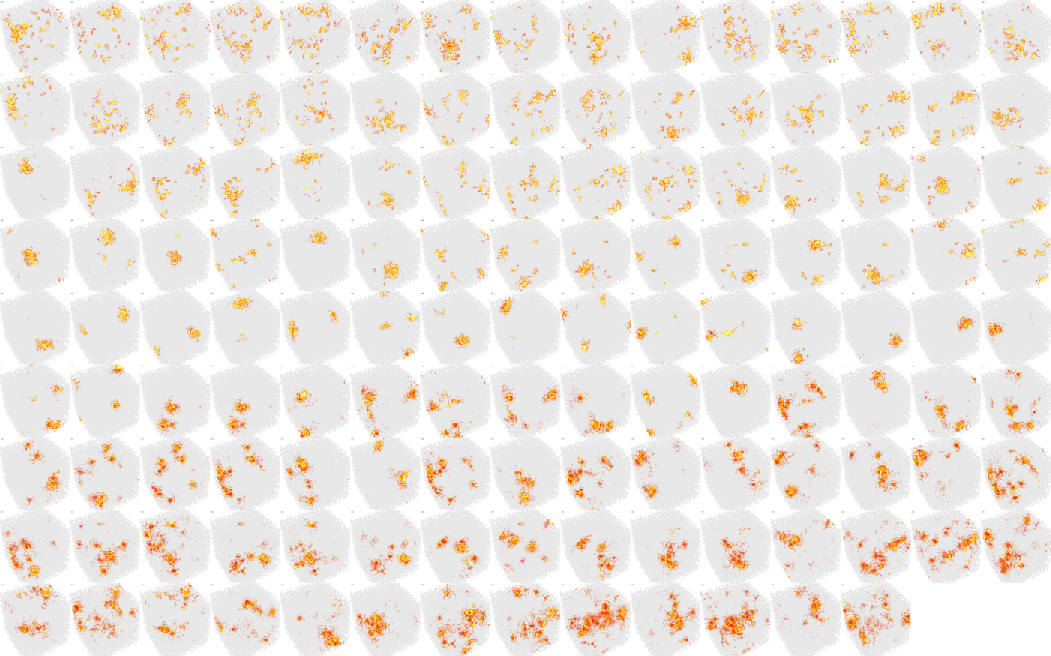
\includegraphics[width=\textwidth]{figS_montage_n10k}
\caption{$N=10^4$: the 133 certified gap-edge modes, 15 per row, in increasing $\lambda$ (labels 4942--5074, see text for the index caveat). Read top to bottom: energy spread over the box (window bottom), collapse to single compact blobs at the gap edges and inside the gap, spreading out again above.}
\label{figS_montage_n10k}
\end{figure}
\begin{figure}
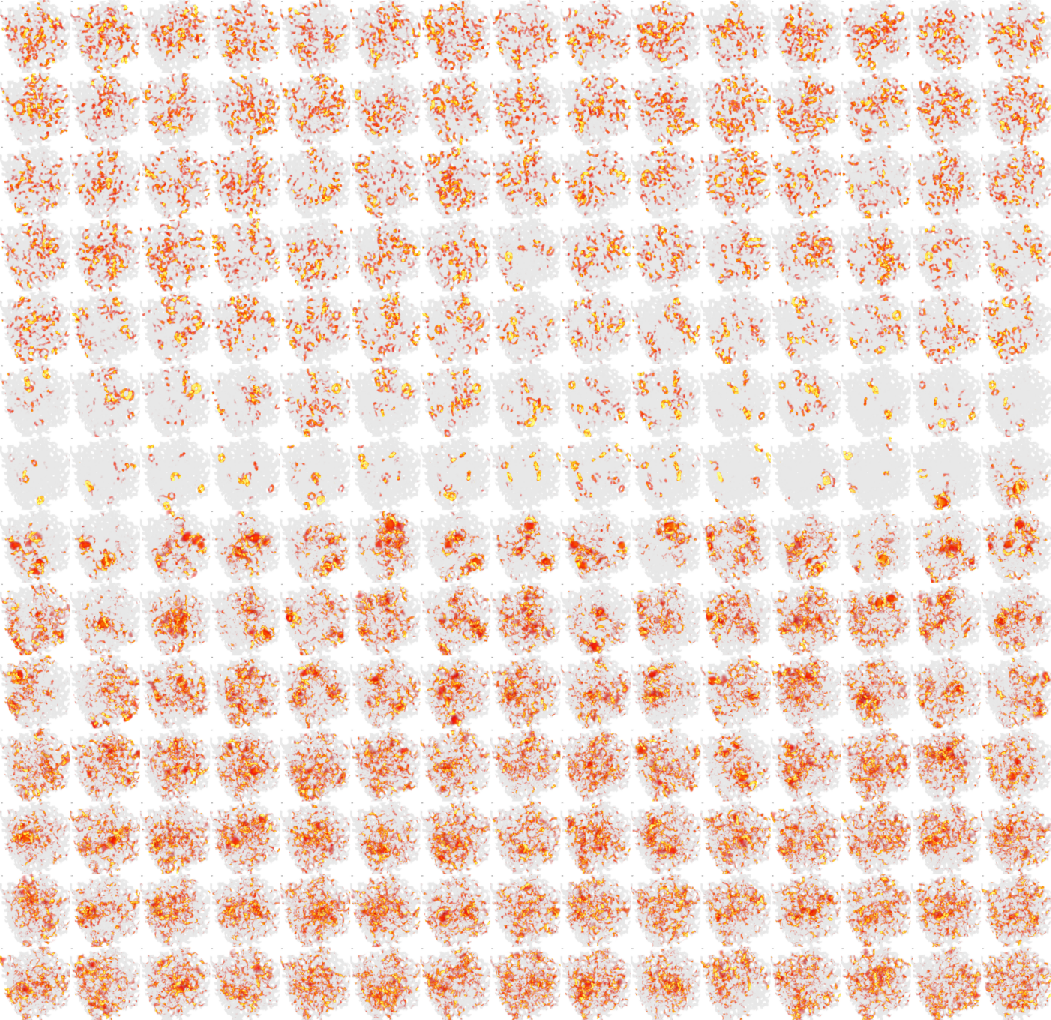
\includegraphics[width=\textwidth]{figS_montage_n1k_circ}
\caption{$N=1000$, circular decoration: 210-tile montage of bands 398--607 for the finite-size comparison with Fig.~\ref{figS_montage_n10k} (same decoration).}
\label{figS_montage_circ}
\end{figure}

\bibliographystyle{apsrev4-2}
\bibliography{refs}
\end{document}
